 \documentclass[12pt,journal,onecolumn]{IEEEtran}
\usepackage[utf8]{inputenc}
\usepackage[T1]{fontenc}
\usepackage[spanish,es-nodecimaldot]{babel}
\usepackage{lmodern}
\usepackage{graphicx}
\usepackage{booktabs}
\usepackage{tabularx}
\usepackage{longtable}
\usepackage{array}
\usepackage{multirow}
\usepackage{xcolor}
\usepackage{float}
\usepackage{placeins}
\usepackage{pdflscape}
\usepackage{enumitem}
\usepackage{hyperref}
\usepackage{url}
\usepackage{fancyvrb}
\usepackage{ragged2e}
\usepackage{microtype}
\usepackage{pifont}
\usepackage{amsmath}

\graphicspath{{images/}}
\hypersetup{colorlinks=true,linkcolor=black,citecolor=black,urlcolor=blue,pdftitle={SIGBUNI - ERS/SRS Entrega 3 (2A)}}
\setlength{\parskip}{0.35em}
\setlength{\parindent}{0pt}
\renewcommand{\arraystretch}{1.18}
\newcolumntype{Y}{>{\RaggedRight\arraybackslash}X}
\newcolumntype{P}[1]{>{\RaggedRight\arraybackslash}p{#1}}
\newcommand{\pendiente}[1]{\textcolor{red!70!black}{\textbf{[PENDIENTE: #1]}}}
\newcommand{\completar}{\textcolor{red!70!black}{\textbf{[COMPLETAR]}}}
\newcommand{\cmark}{\ding{51}}
\newcommand{\xmark}{\ding{55}}
\newcommand{\placeholderfigure}[2]{%
\begin{figure}[H]\centering
\fbox{\parbox[c][#2][c]{0.92\textwidth}{\centering\bfseries #1\\[0.5em]\normalfont Inserte aquí el archivo PNG/SVG exportado desde la herramienta de modelado y mantenga el archivo fuente editable en el repositorio.}}
\caption{#1}\end{figure}}
\newcommand{\reqblock}[9]{%
\medskip\noindent\textbf{#1 --- #2}\par\smallskip
\begin{tabularx}{\textwidth}{P{0.19\textwidth}Y}\toprule
\textbf{ID} & #1\\
\textbf{Nombre} & #2\\
\textbf{Descripción} & #3\\
\textbf{Actor principal} & #4\\
\textbf{Entrada} & #5\\
\textbf{Proceso} & #6\\
\textbf{Salida} & #7\\
\textbf{Prioridad MoSCoW} & #8\\
\textbf{Evidencia} & #9\\\bottomrule
\end{tabularx}\par\medskip}
\newcommand{\caseblock}[9]{%
\medskip\noindent\textbf{#1 --- #2}\par\smallskip
\begin{tabularx}{\textwidth}{P{0.19\textwidth}Y}\toprule
\textbf{Actor principal} & #3\\
\textbf{Objetivo} & #4\\
\textbf{Precondiciones} & #5\\
\textbf{Flujo principal} & #6\\
\textbf{Flujo alternativo} & #7\\
\textbf{Poscondiciones} & #8\\
\textbf{Requisitos relacionados} & #9\\\bottomrule
\end{tabularx}\par\medskip}
\newcommand{\blankreq}[1]{\reqblock{#1}{\completar}{\completar}{\completar}{\completar}{\completar}{\completar}{\completar}{\completar}}
\newcommand{\blankcase}[2]{\caseblock{#1}{#2}{\completar}{\completar}{\completar}{\completar}{\completar}{\completar}{\completar}}

\begin{document}
\title{SIGBUNI: Especificación de Requisitos Completa y Protocolo Empírico\\Entrega 3 (2A)}
\author{Cedeño Coronado Wilson Lizandro y Chavarria Cuenca Tahiny Mel\\
Universidad Técnica Estatal de Quevedo, Facultad de Ciencias de la Computación\\
Asignatura: Ingeniería de Requerimientos --- Docente: Ing. Guerrero Ulloa Gleiston}
\maketitle

\begin{abstract}
Este documento consolida la Especificación de Requisitos de Software del Sistema Inteligente de Gestión Bibliotecaria Universitaria (SIGBUNI) y estructura los elementos exigidos para la Entrega 3 (2A). Se reutiliza únicamente la información documentada en las entregas 1A y 2 (1B): contexto, alcance, actores, requisitos, interfaces, mockups, modelos UML, priorización y trazabilidad inicial. Los apartados que requieren nueva evidencia de campo, validación, métricas legales, historias de usuario, criterios de aceptación, modelos adicionales, MVP, registro OSF, resultados experimentales o datos FAIR se presentan como plantillas identificadas explícitamente como pendientes. Esta separación evita declarar como completada información que todavía no posee respaldo empírico verificable y facilita la actualización del documento desde un único archivo LaTeX basado en la clase IEEEtran.
\end{abstract}

\begin{IEEEkeywords}
Ingeniería de Requerimientos, biblioteca universitaria, SIGBUNI, inteligencia artificial, trazabilidad, estudio empírico.
\end{IEEEkeywords}

\begin{center}
\textbf{Repositorio documental:} \url{https://github.com/TahinyMel/SIGBUNI_ISR401}
\end{center}

\section*{Historial de versiones}
\begin{tabularx}{\textwidth}{P{0.11\textwidth}P{0.15\textwidth}P{0.18\textwidth}Y}\toprule
\textbf{Versión} & \textbf{Fecha} & \textbf{Responsable} & \textbf{Descripción}\\\midrule
0.1 & 2026 & Equipo SIGBUNI & Planificación y elicitación de requisitos (Entrega 1A).\\
0.2 & 03/07/2026 & Equipo SIGBUNI & ERS/SRS parcial, requisitos refinados, interfaces, UML y trazabilidad inicial (Entrega 2/1B).\\
1.0-borrador & 19/07/2026 & Equipo SIGBUNI & Migración a IEEEtran y estructura completa de la Entrega 3 (2A), con plantillas para información aún no respaldada.\\\bottomrule
\end{tabularx}

\vspace{1em}
\textbf{Firma electrónica del analista líder:} \pendiente{insertar firma electrónica verificable antes del corte}.

\tableofcontents
\listoffigures
\listoftables
\clearpage

\section{Introducción}
\subsection{Propósito del documento}
El propósito de este documento es presentar la ERS/SRS completa de SIGBUNI y organizar, en un único artefacto verificable, los requisitos, modelos, evidencias, protocolos y productos solicitados para la Entrega 3 (2A). El documento toma como línea base las Entregas 1A y 2 (1B) del proyecto \cite{sigbuni1a2026,sigbuni1b2026}, y adopta como referencias de estructura ISO/IEC/IEEE 29148:2018 \cite{iso29148_2018}, ISO/IEC 25010:2023 \cite{iso25010_2023}, SWEBOK v4.0 \cite{swebok2024} y Pohl \cite{pohl2010}.

\subsection{Alcance del producto}
SIGBUNI se concibe como una aplicación web responsiva para centralizar los servicios bibliotecarios universitarios. El producto digitaliza procesos actualmente manuales o desarticulados, especialmente préstamo y devolución de materiales, consulta de catálogo, reserva de espacios, control de acceso, notificaciones, asistencia mediante IA e informes para toma de decisiones.

\begin{table}[H]\centering
\caption{Alcance del producto}
\begin{tabularx}{\textwidth}{Y Y}\toprule
\textbf{Incluido en el alcance} & \textbf{Fuera del alcance}\\\midrule
Gestión de préstamos, devoluciones y renovaciones físicas. & Administración financiera o cobro directo de multas.\\
Reserva digital de cubículos, salas y otros espacios. & Integración con sistemas de pago universitario.\\
Control de acceso con registro digital de entrada y salida. & Gestión de adquisición de nuevos materiales.\\
Catálogo digital con búsqueda avanzada y estado actualizado. & Administración de dependencias ajenas a la biblioteca.\\
Asistente IA para recomendación, consultas y apoyo académico. & Plataforma de aprendizaje en línea (LMS).\\
Notificaciones internas por préstamos, reservas y comunicados. & Digitalización completa del acervo bibliográfico físico.\\
Reportes estadísticos de servicios, aforo y demanda. & Biblioteca digital externa o repositorios académicos de terceros.\\\bottomrule
\end{tabularx}
\end{table}

\subsection{Objetivos del sistema}
\textbf{Objetivo general:} Diseñar y documentar los requisitos de un sistema centralizado para la gestión de los servicios bibliotecarios universitarios, incorporando componentes de IA para mejorar la eficiencia operativa, la disponibilidad de información y la experiencia de los usuarios.

\begin{enumerate}[label=OBJ-\arabic*]
\item Digitalizar y agilizar los procesos de préstamo, devolución y renovación.
\item Especificar la reserva en línea de cubículos, salas y otros espacios.
\item Definir el control de acceso y el registro de entradas y salidas.
\item Mantener un catálogo digital consultable y actualizado en tiempo real.
\item Incorporar asistencia inteligente para recomendación y apoyo académico.
\item Generar reportes estadísticos para decisiones administrativas e institucionales.
\end{enumerate}

\subsection{Definiciones, acrónimos y abreviaturas}
\begin{longtable}{P{0.18\textwidth}P{0.76\textwidth}}\toprule
\textbf{Término} & \textbf{Definición}\\\midrule\endfirsthead
\toprule\textbf{Término} & \textbf{Definición}\\\midrule\endhead
ERS/SRS & Especificación de Requisitos de Software.\\
IA & Inteligencia Artificial.\\
SIGBUNI & Sistema Inteligente de Gestión Bibliotecaria Universitaria.\\
Stakeholder & Persona, grupo o área con interés, influencia o participación en el sistema.\\
RF / RNF / RD & Requisito funcional / requisito no funcional / restricción de diseño.\\
EV & Identificador de evidencia primaria verificable.\\
CU / HU / CA & Caso de uso / historia de usuario / criterio de aceptación.\\
MoSCoW & Priorización Must, Should, Could y Won't have.\\
Kano & Clasificación de atributos según su efecto en la satisfacción.\\
WSJF & Weighted Shortest Job First; priorización por costo de retraso y tamaño del trabajo.\\
MVP & Producto Mínimo Viable.\\
OSF & Open Science Framework.\\
FAIR & Principios de datos localizables, accesibles, interoperables y reutilizables.\\
\bottomrule
\end{longtable}

\subsection{Referencias y control bibliográfico}
La bibliografía se administra en \texttt{referencias.bib}. La rúbrica exige al menos 25 fuentes primarias y al menos 10 publicadas en los tres años anteriores al corte. El archivo adjunto contiene las fuentes base citadas por la guía y por las entregas previas; antes de la entrega se debe verificar cada registro en Scopus o Web of Science, completar DOI y sustituir o agregar las fuentes recientes necesarias. No se debe declarar el cumplimiento de ese mínimo sin la comprobación documental correspondiente.

\subsection{Visión general del documento}
Las Secciones 1 a 6 constituyen la ERS/SRS. Las Secciones 7 a 10 integran el trabajo de campo, el protocolo experimental, la preparación de publicación y el control del repositorio. Los apartados marcados como \completar requieren evidencia nueva y no deben considerarse finalizados hasta que los artefactos correspondientes estén versionados en GitHub.

\section{Descripción general}
\subsection{Perspectiva del producto y límite del sistema}
SIGBUNI será un punto único para autenticación, catálogo, préstamos, reservas, control de acceso, IA, notificaciones, reportes y administración. Se excluyen pagos, plataformas LMS, repositorios externos y procesos institucionales no relacionados con la biblioteca.

\begin{figure}[H]\centering
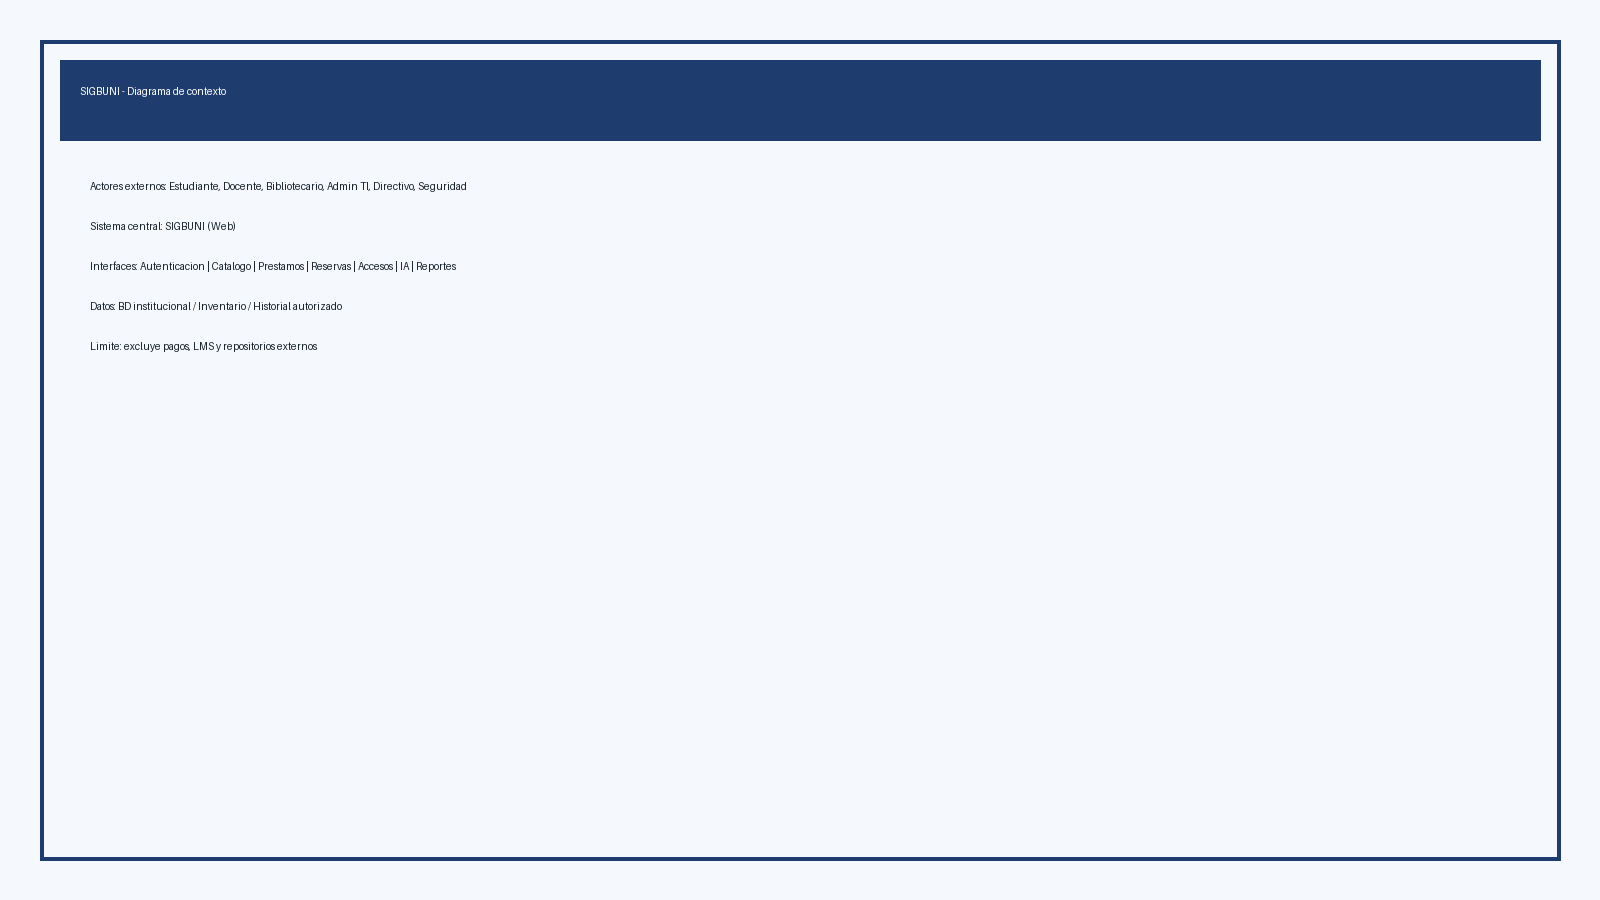
\includegraphics[width=0.96\textwidth]{diagrama_contexto.png}
\caption{Diagrama de contexto heredado de la Entrega 2 (1B).}
\label{fig:contexto}
\end{figure}

\subsection{Funciones del producto}
\begin{longtable}{P{0.12\textwidth}P{0.82\textwidth}}\toprule
\textbf{ID} & \textbf{Función de alto nivel}\\\midrule\endfirsthead
\toprule\textbf{ID} & \textbf{Función de alto nivel}\\\midrule\endhead
FP-01 & Gestionar préstamo, devolución y renovación de materiales.\\
FP-02 & Mantener un catálogo digital actualizado y consultable.\\
FP-03 & Permitir la reserva digital de espacios físicos.\\
FP-04 & Registrar ingreso y salida mediante control de acceso.\\
FP-05 & Gestionar usuarios, roles y permisos.\\
FP-06 & Enviar notificaciones internas.\\
FP-07 & Atender consultas frecuentes mediante chatbot.\\
FP-08 & Recomendar materiales según carrera, historial o tema.\\
FP-09 & Generar resúmenes automáticos cuando aplique.\\
FP-10 & Generar reportes estadísticos de uso, demanda y aforo.\\\bottomrule
\end{longtable}

\subsection{Clases y características de usuarios}
\begin{table}[H]\centering
\caption{Perfiles de usuario}
\begin{tabularx}{\textwidth}{P{0.20\textwidth}Y Y}\toprule
\textbf{Usuario} & \textbf{Características} & \textbf{Funciones principales}\\\midrule
Estudiante & Usuario frecuente que requiere acceso rápido al catálogo, préstamos, reservas, alertas y orientación. & Consultar catálogo, solicitar préstamos, reservar espacios, usar chatbot y recibir alertas.\\
Docente / investigador & Requiere materiales especializados, espacios y recomendaciones por área. & Buscar material, reservar salas, recibir recomendaciones y consultar disponibilidad.\\
Personal de biblioteca & Opera procesos diarios y mantiene la información actualizada. & Registrar préstamos, devoluciones, accesos, inventario y reportes.\\
Administrador TI & Configura seguridad, usuarios, permisos y soporte. & Gestionar roles, parámetros, respaldos e integraciones.\\
Directivo académico & Consulta información para toma de decisiones. & Visualizar reportes de demanda, aforo y uso.\\\bottomrule
\end{tabularx}
\end{table}

\subsection{Mapa de stakeholders}
\begin{table}[H]\centering
\caption{Matriz poder/interés}
\begin{tabularx}{\textwidth}{P{0.10\textwidth}P{0.28\textwidth}P{0.12\textwidth}P{0.12\textwidth}Y}\toprule
\textbf{ID} & \textbf{Stakeholder} & \textbf{Poder} & \textbf{Interés} & \textbf{Estrategia}\\\midrule
S-01 & Estudiantes & Alto & Alto & Gestionar de cerca y validar facilidad de uso.\\
S-02 & Docentes e investigadores & Alto & Medio & Consultar periódicamente.\\
S-03 & Personal de biblioteca & Alto & Alto & Gestionar de cerca por su criticidad operativa.\\
S-04 & Decanos y directivos & Medio & Bajo & Informar avances y entregar reportes ejecutivos.\\
S-05 & Área de TI & Alto & Medio & Mantener satisfecha y validar infraestructura y seguridad.\\
S-06 & Rectoría / Dirección académica & Alto & Bajo & Mantener informada como patrocinador institucional.\\\bottomrule
\end{tabularx}
\end{table}

\subsection{Entorno operativo}
El sistema operará como una aplicación web responsiva accesible desde navegadores modernos en computadoras, laptops, tabletas y teléfonos. El personal administrativo empleará estaciones de trabajo dentro de la biblioteca. El control de acceso podrá apoyarse en lector QR, cámara o credencial institucional, según la infraestructura disponible. Los datos se almacenarán en una base centralizada gestionada por TI.

\subsection{Suposiciones y dependencias}
\begin{longtable}{P{0.12\textwidth}P{0.28\textwidth}P{0.54\textwidth}}\toprule
\textbf{ID} & \textbf{Suposición/dependencia} & \textbf{Descripción}\\\midrule\endfirsthead
\toprule\textbf{ID} & \textbf{Suposición/dependencia} & \textbf{Descripción}\\\midrule\endhead
SD-01 & Conectividad institucional & Conexión estable a internet o red universitaria.\\
SD-02 & Datos actualizados & Catálogo e inventario mantenidos por personal autorizado.\\
SD-03 & Credenciales & Identificación universitaria válida.\\
SD-04 & Infraestructura TI & Servidor, base de datos, respaldo y mantenimiento.\\
SD-05 & Servicios de IA & Disponibilidad y configuración del módulo de IA.\\
SD-06 & Capacitación & Formación del personal para adoptar el flujo digital.\\\bottomrule
\end{longtable}

\subsection{Modelado organizacional i*}
La rúbrica exige un Diagrama de Dependencia Estratégica (SD) y un Diagrama de Razón Estratégica (SR). Estos modelos no constan en las entregas previas.
\placeholderfigure{Diagrama i* de Dependencia Estratégica (SD)}{5cm}
\placeholderfigure{Diagrama i* de Razón Estratégica (SR)}{5cm}

\section{Requisitos específicos completos}
\subsection{Interfaces externas}
\medskip\noindent\textbf{Interfaces de usuario}\par\smallskip
\begin{table}[H]\centering
\caption{Interfaces de usuario identificadas}
\begin{tabularx}{\textwidth}{P{0.12\textwidth}P{0.25\textwidth}Y}\toprule
\textbf{ID} & \textbf{Interfaz} & \textbf{Descripción}\\\midrule
IU-01 & Inicio de sesión & Autenticación con credenciales institucionales y validación de rol.\\
IU-02 & Catálogo digital & Búsqueda por título, autor, ISBN, área, carrera y estado.\\
IU-03 & Reserva de espacios & Selección de fecha, horario, espacio y confirmación.\\
IU-04 & Chatbot IA & Preguntas sobre servicios y orientación académica.\\
IU-05 & Panel bibliotecario & Gestión de préstamos, devoluciones, inventario, accesos y reportes.\\\bottomrule
\end{tabularx}
\end{table}

\begin{figure}[H]\centering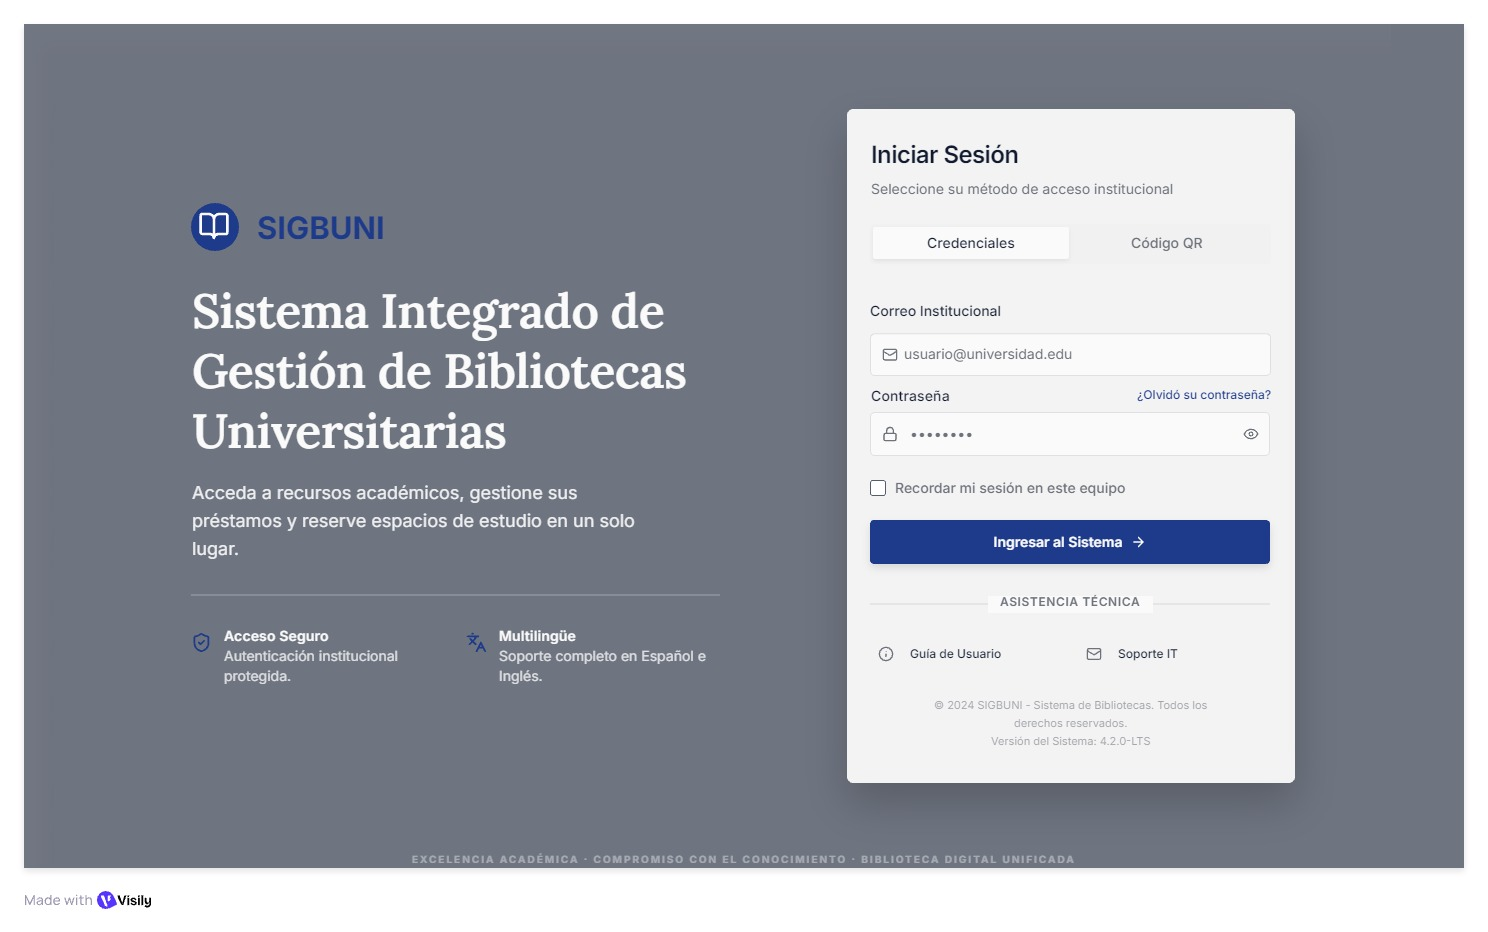
\includegraphics[width=0.82\textwidth]{MU-01_inicio_sesion.png}\caption{MU-01: mockup inicial de inicio de sesión.}\end{figure}
\begin{figure}[H]\centering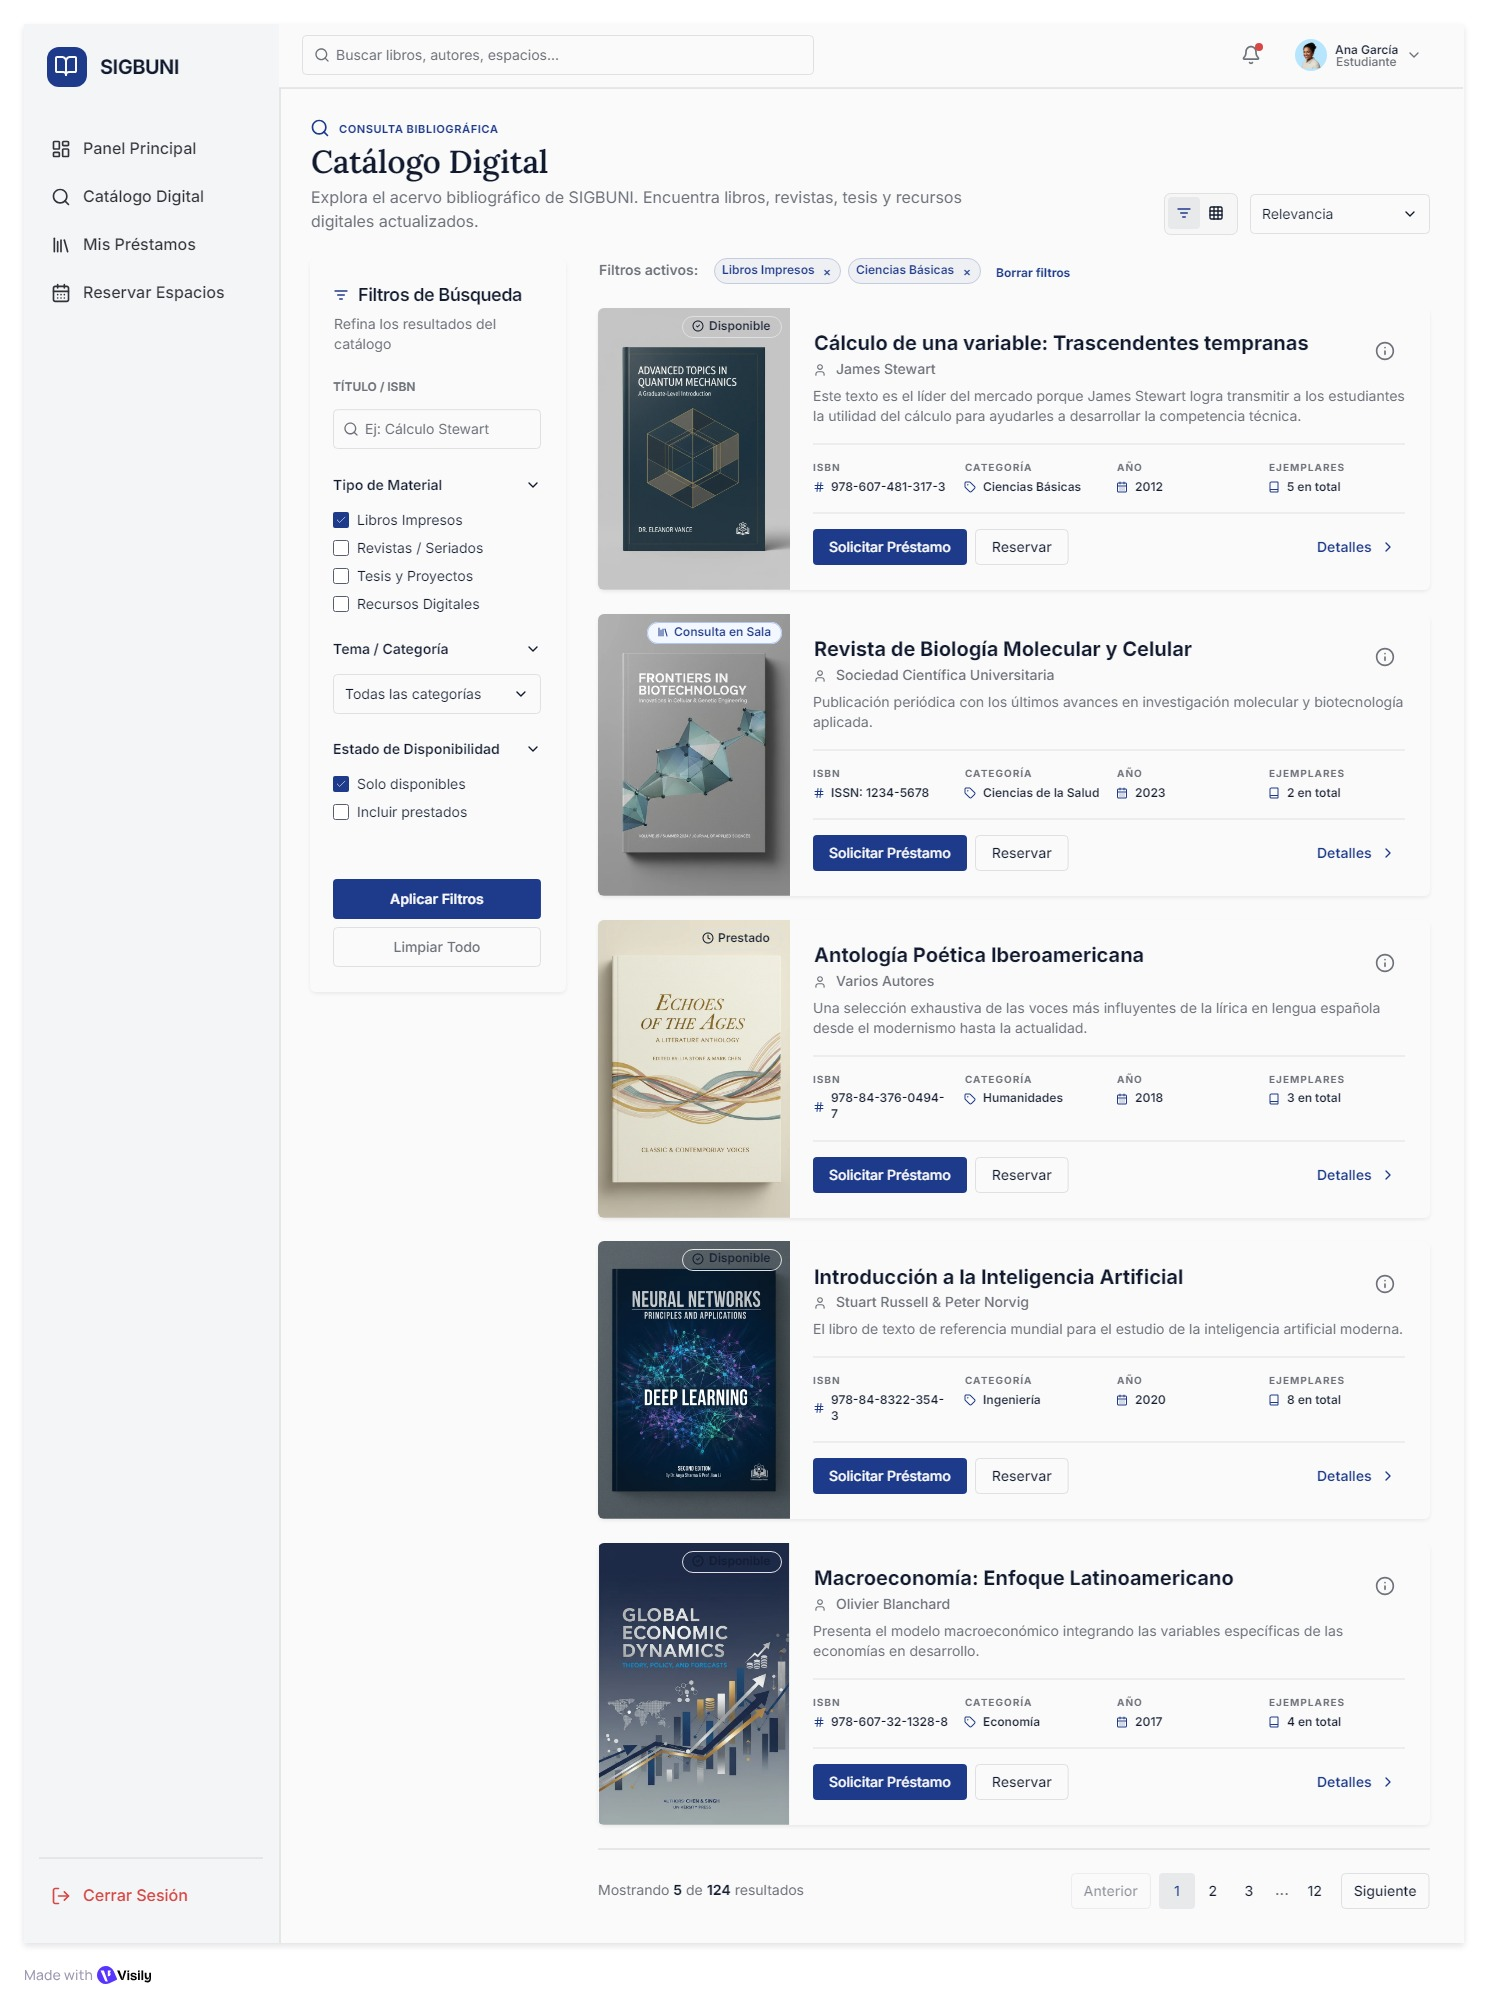
\includegraphics[width=0.82\textwidth]{MU-02_catalogo.png}\caption{MU-02: mockup inicial del catálogo digital.}\end{figure}
\begin{figure}[H]\centering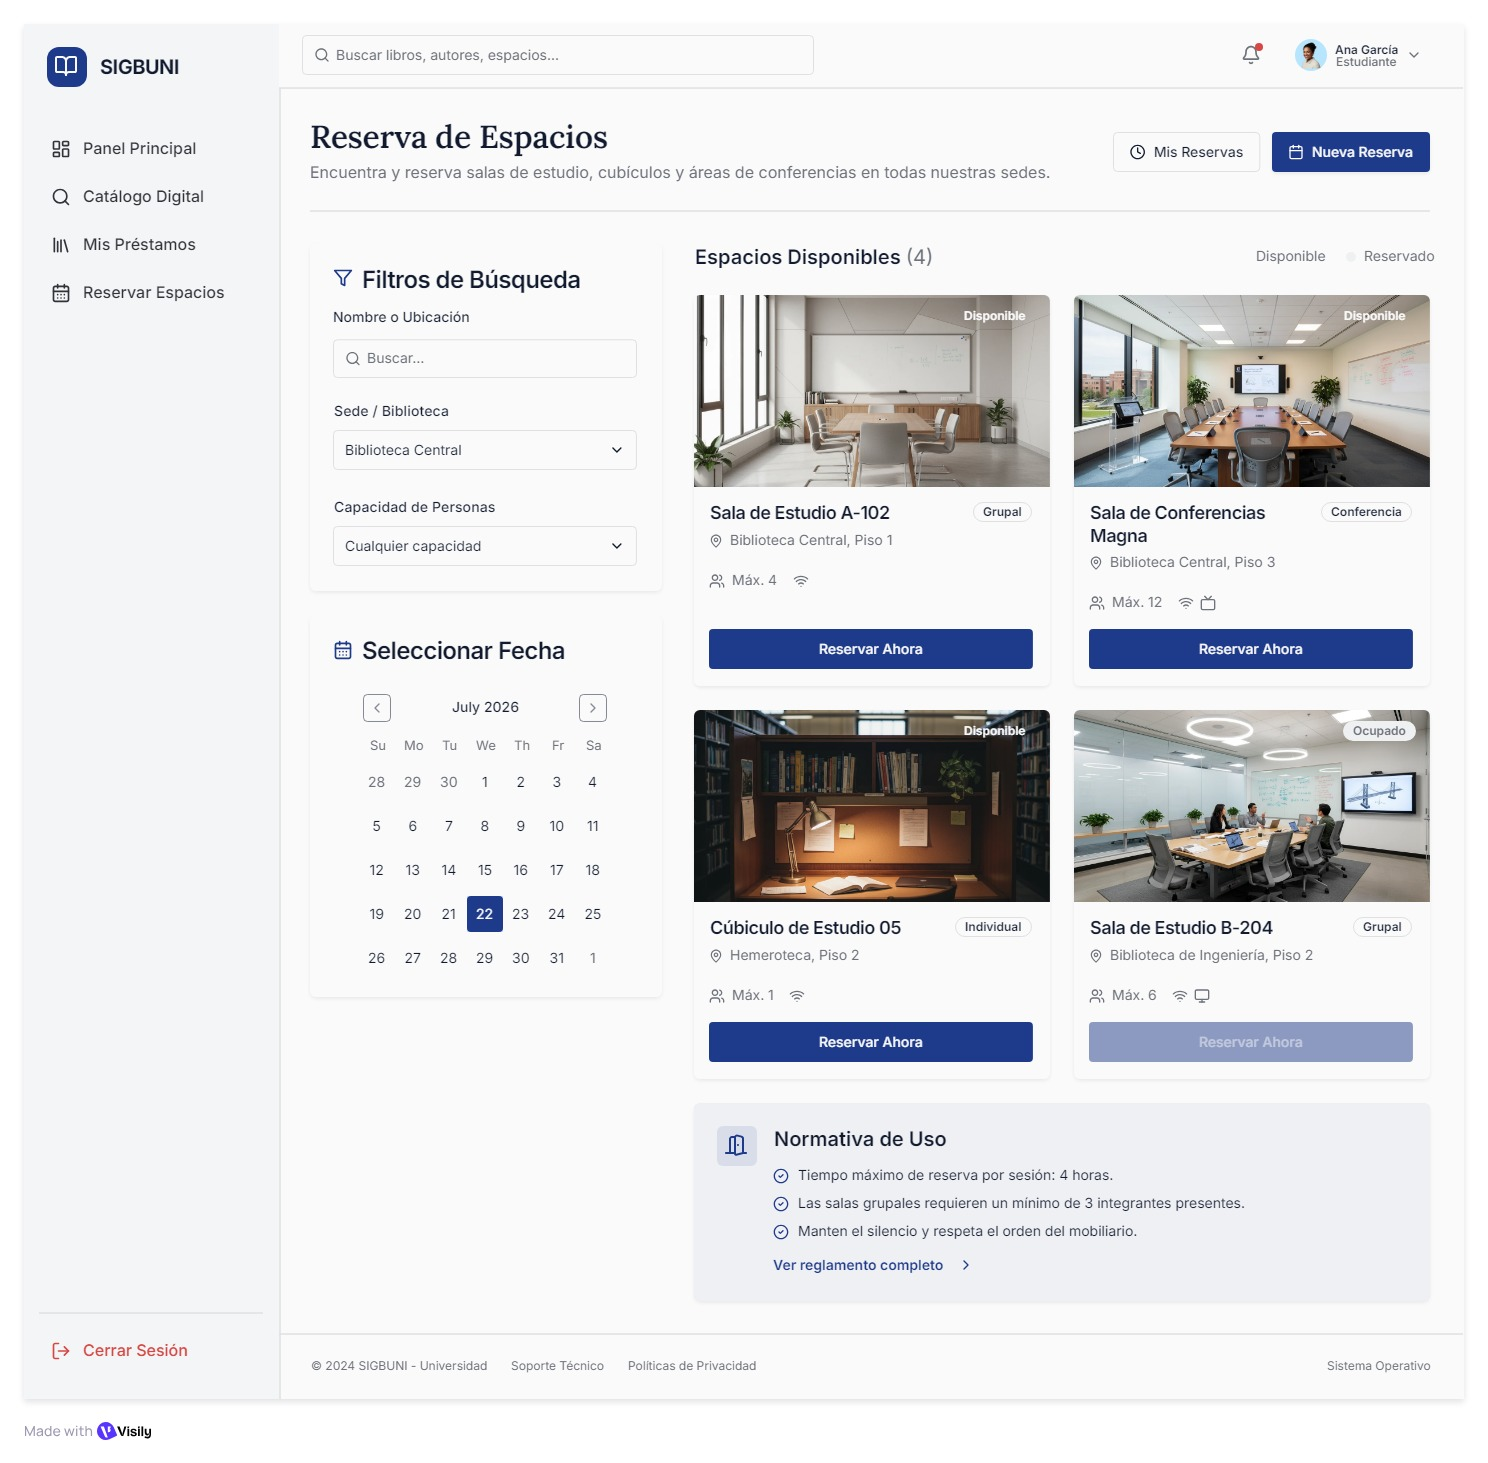
\includegraphics[width=0.82\textwidth]{MU-03_reserva_espacios.png}\caption{MU-03: mockup inicial de reserva de espacios.}\end{figure}
\begin{figure}[H]\centering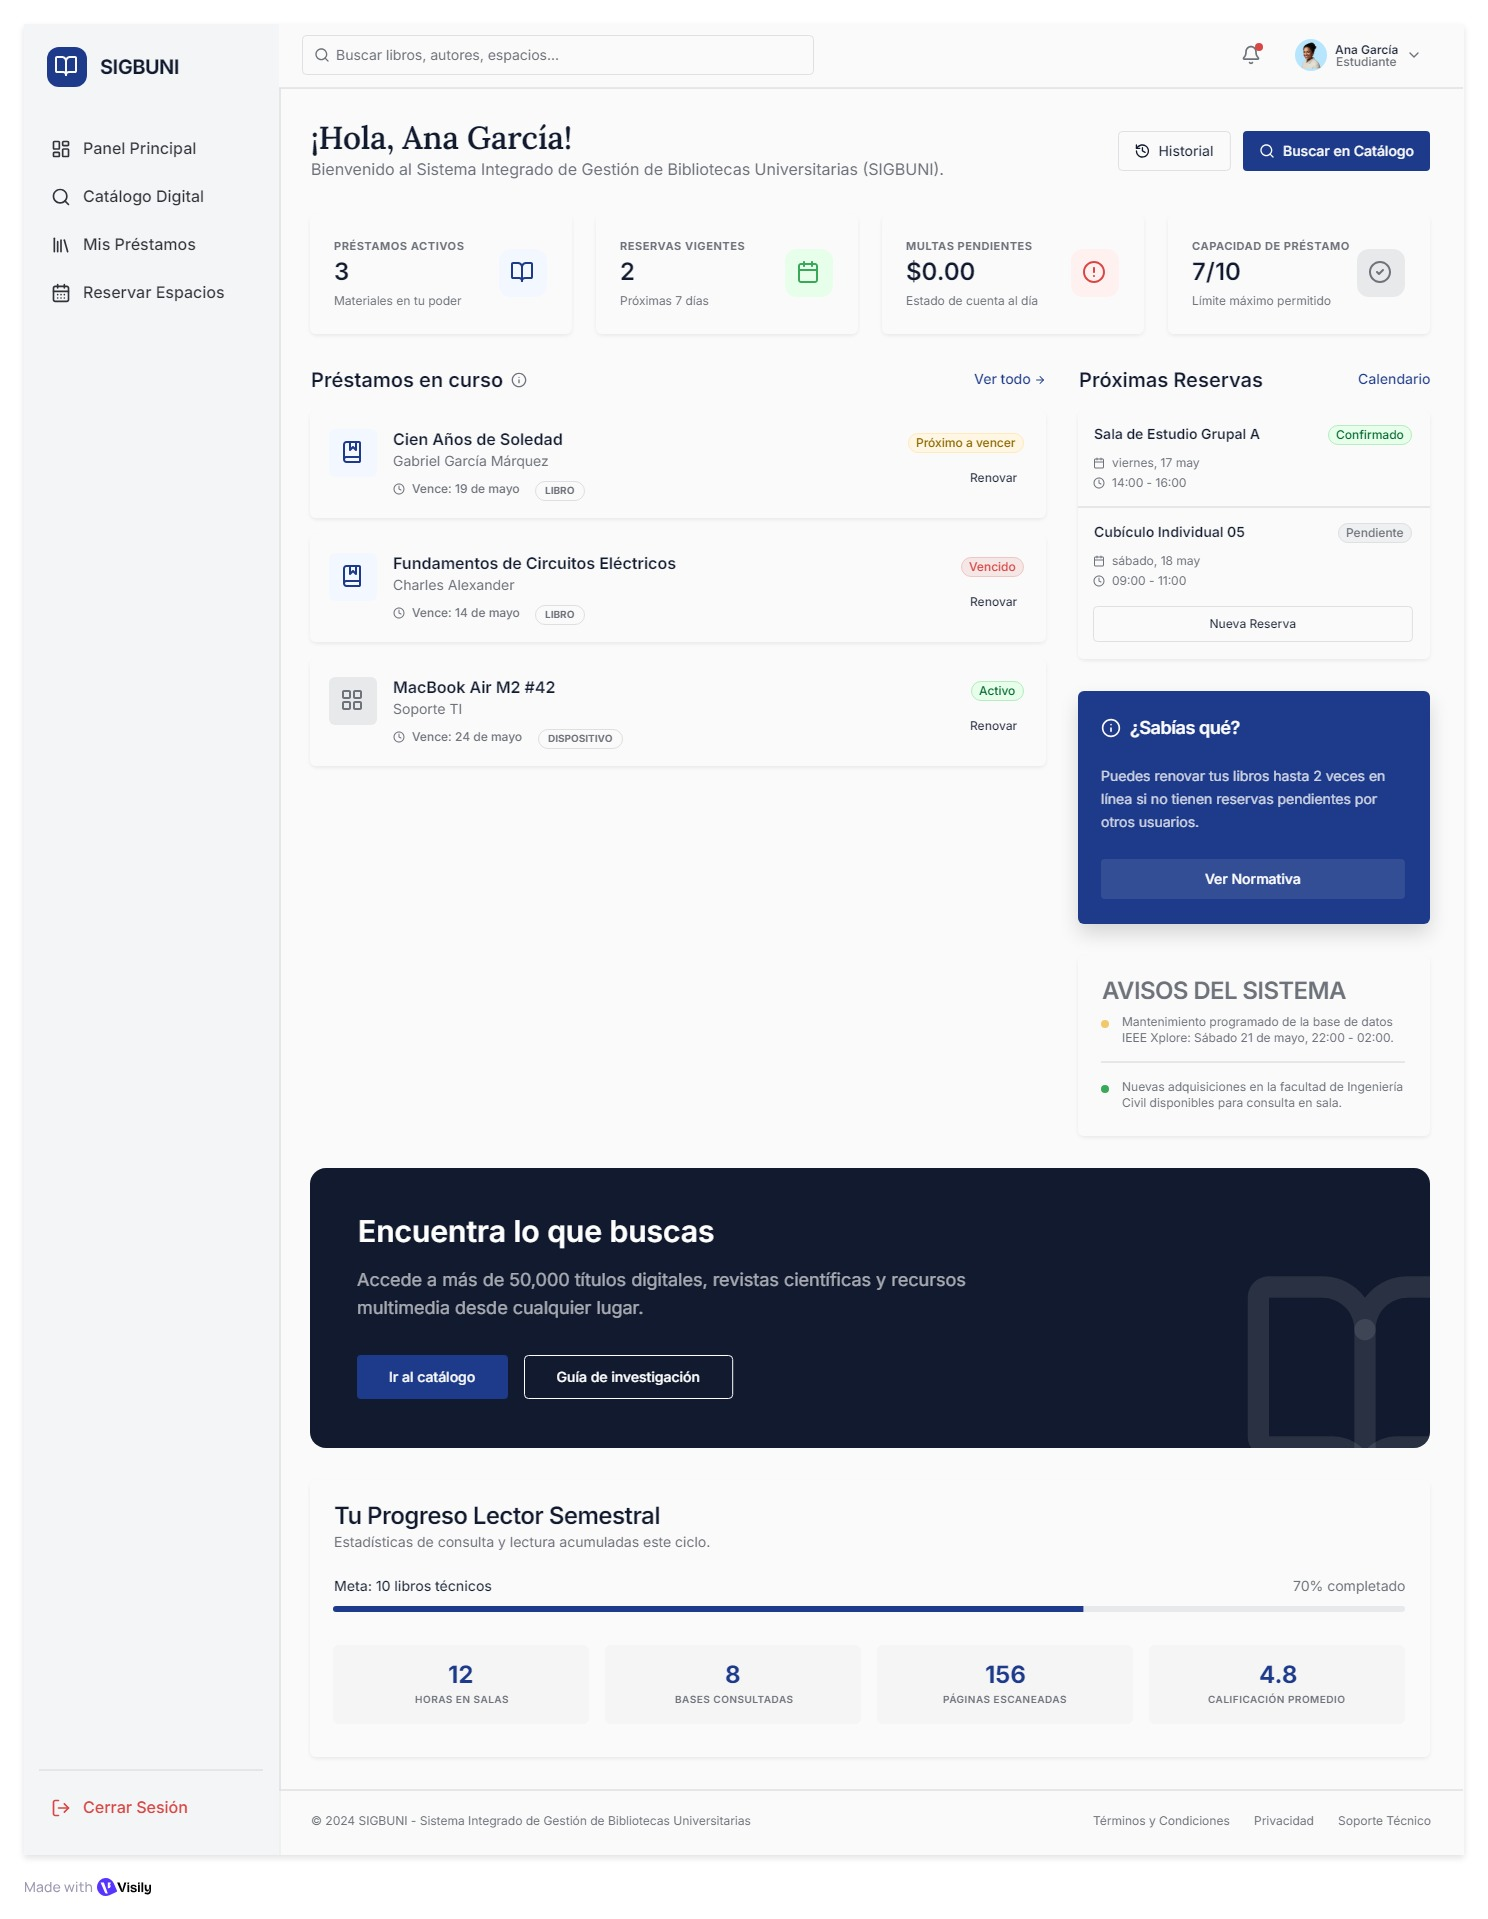
\includegraphics[width=0.82\textwidth]{MU-04_chatbot.png}\caption{MU-04: mockup inicial del chatbot.}\end{figure}
\begin{figure}[H]\centering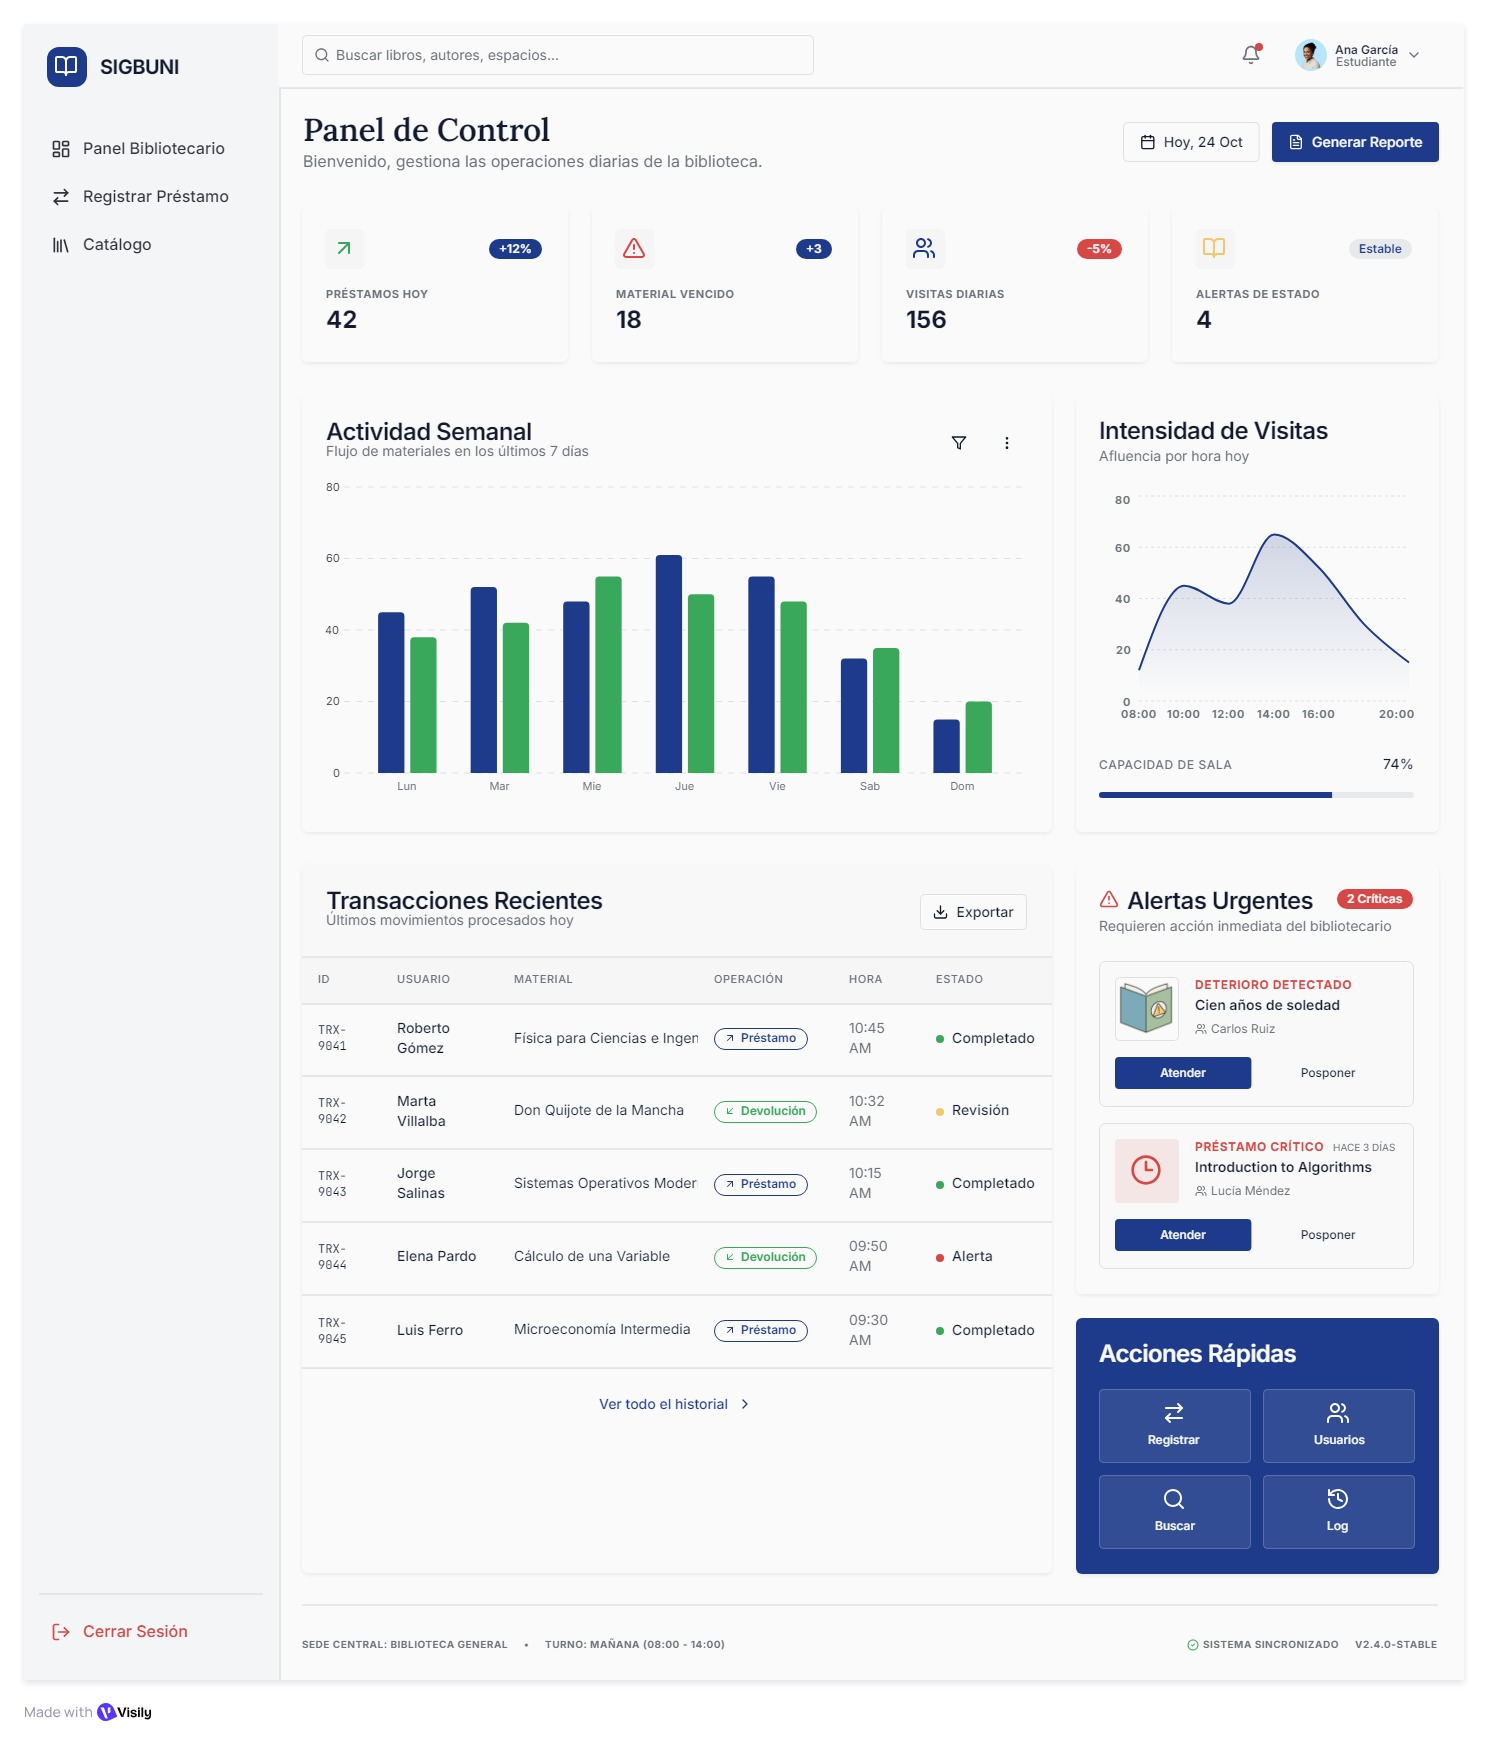
\includegraphics[width=0.82\textwidth]{MU-05_panel_bibliotecario.png}\caption{MU-05: mockup inicial del panel bibliotecario.}\end{figure}

\begin{table}[H]\centering
\caption{Trazabilidad inicial de mockups}
\begin{tabularx}{\textwidth}{P{0.13\textwidth}P{0.28\textwidth}Y P{0.16\textwidth}}\toprule
\textbf{Mockup} & \textbf{Pantalla} & \textbf{RF soportados} & \textbf{Estado}\\\midrule
MU-01 & Inicio de sesión & RF-17 y RNF de seguridad/autorización & Baseline; elevar a alta fidelidad.\\
MU-02 & Catálogo digital & RF-06, RF-07, RF-08 & Baseline; elevar a alta fidelidad.\\
MU-03 & Reserva de espacios & RF-09, RF-10, RF-11 & Baseline; elevar a alta fidelidad.\\
MU-04 & Chatbot IA & RF-04, RF-14, RF-15, RF-16, RF-20 & Baseline; elevar a alta fidelidad y agregar explicación.\\
MU-05 & Panel bibliotecario & RF-01, RF-02, RF-05, RF-17, RF-18, RF-19 & Baseline; elevar a alta fidelidad.\\
MU-06--MU-XX & Pantallas Must no cubiertas & \completar & \completar\\\bottomrule
\end{tabularx}
\end{table}

\medskip\noindent\textbf{Interfaces de hardware}\par\smallskip
\begin{tabularx}{\textwidth}{P{0.30\textwidth}Y}\toprule
\textbf{Hardware} & \textbf{Uso}\\\midrule
Lector QR o cámara & Verificar credencial y registrar ingreso/salida.\\
Computadoras administrativas & Operar préstamos, devoluciones, inventario y reportes.\\
Servidor institucional & Alojar aplicación, base de datos y servicios.\\
Dispositivos móviles & Acceder a catálogo, reservas y chatbot.\\\bottomrule
\end{tabularx}

\medskip\noindent\textbf{Interfaces de software}\par\smallskip
\begin{tabularx}{\textwidth}{P{0.30\textwidth}Y}\toprule
\textbf{Software/servicio} & \textbf{Uso}\\\midrule
Base de datos centralizada & Almacenar usuarios, materiales, préstamos, reservas, accesos y notificaciones.\\
Módulo de IA & Procesar recomendaciones, consultas y resúmenes.\\
Servicio de autenticación & Validar credenciales y acceso por rol.\\
Notificaciones internas & Emitir alertas y comunicados.\\
GitHub & Versionar documentación, diagramas, evidencias y código.\\\bottomrule
\end{tabularx}

\subsection{Requisitos funcionales}
Los RF-01 a RF-20 se transcriben y reorganizan a partir de la Entrega 2 (1B). Se incorpora el campo de evidencia con base en la matriz de trazabilidad previa. Los RF-21 a RF-25 quedan como plantillas porque aún no existen requisitos respaldados para completar el mínimo exigido.
\reqblock{RF-01}{Registrar préstamo bibliográfico}{El sistema debe permitir registrar el préstamo de un material bibliográfico a un usuario autorizado.}{Personal administrativo de biblioteca}{Código del usuario, código del material, fecha de préstamo y fecha esperada de devolución.}{Validar al usuario, verificar la disponibilidad, registrar el préstamo y cambiar el estado del material a prestado.}{Préstamo registrado y disponibilidad actualizada.}{Must}{EV-01, EV-15}
\reqblock{RF-02}{Registrar devolución de material}{El sistema debe permitir registrar la devolución de un material prestado.}{Personal administrativo de biblioteca}{Código del préstamo o material devuelto.}{Validar el préstamo activo, registrar la fecha real de devolución y actualizar el estado del material.}{Devolución registrada y material disponible o marcado según condición.}{Must}{EV-01}
\reqblock{RF-03}{Renovar préstamo digitalmente}{El sistema debe permitir renovar préstamos vigentes cuando no existan reservas pendientes del material.}{Estudiante / docente}{Solicitud de renovación y préstamo activo.}{Verificar vigencia, ausencia de reservas y límite de renovaciones; actualizar la fecha de devolución.}{Préstamo renovado o solicitud rechazada con motivo.}{Should}{EV-10}
\reqblock{RF-04}{Enviar notificación de vencimiento}{El sistema debe notificar al usuario cuando la fecha de devolución esté próxima a vencer.}{Sistema de notificaciones}{Préstamos próximos a vencer.}{Identificar préstamos con vencimiento cercano y generar una alerta interna al iniciar sesión.}{Notificación visible para el usuario.}{Must}{EV-01, EV-08}
\reqblock{RF-05}{Generar alerta por material vencido}{El sistema debe alertar al personal cuando un material no sea devuelto dentro del plazo establecido.}{Sistema / bibliotecario}{Fecha de devolución esperada vencida.}{Comparar la fecha actual con la fecha esperada y generar una alerta administrativa.}{Alerta de material vencido en el panel bibliotecario.}{Must}{EV-01}
\reqblock{RF-06}{Consultar catálogo digital}{El sistema debe permitir consultar el catálogo digital de materiales bibliográficos.}{Estudiante / docente / bibliotecario}{Criterio general de búsqueda.}{Recuperar materiales coincidentes desde la base de datos.}{Listado de materiales encontrados.}{Must}{EV-02, EV-13}
\reqblock{RF-07}{Buscar material por filtros}{El sistema debe permitir filtrar materiales por título, autor, ISBN, área temática, carrera o facultad afín.}{Usuario general}{Filtros seleccionados.}{Aplicar filtros y ordenar resultados según coincidencia.}{Resultados filtrados y legibles.}{Must}{EV-02}
\reqblock{RF-08}{Mostrar estado del material}{El sistema debe mostrar el estado actual de cada material: disponible, prestado, reservado, en mantenimiento o extraviado.}{Usuario general}{Selección o consulta de material.}{Consultar el inventario y presentar el estado actualizado.}{Estado visible del material.}{Must}{EV-02}
\reqblock{RF-09}{Reservar espacio bibliotecario}{El sistema debe permitir reservar cubículos, salas de estudio u otros espacios disponibles.}{Estudiante / docente}{Fecha, hora, espacio, usuario y motivo.}{Verificar disponibilidad y reglas de uso; registrar la reserva.}{Reserva confirmada o rechazada con motivo.}{Must}{EV-03, EV-15}
\reqblock{RF-10}{Mostrar disponibilidad de espacios}{El sistema debe mostrar en tiempo real los espacios disponibles para reserva.}{Usuario general}{Fecha y horario consultado.}{Consultar agenda de espacios y reservas vigentes.}{Calendario o listado de espacios disponibles.}{Must}{EV-03}
\reqblock{RF-11}{Liberar reserva por inasistencia}{El sistema debe liberar automáticamente una reserva si el usuario no se presenta en el tiempo límite configurado.}{Sistema}{Reserva confirmada y tiempo de tolerancia.}{Verificar la ausencia de confirmación de uso y cambiar el estado de la reserva.}{Espacio liberado y disponible para otros usuarios.}{Should}{EV-03}
\reqblock{RF-12}{Registrar ingreso a biblioteca}{El sistema debe registrar el ingreso del usuario al edificio mediante credencial, carnet o código QR.}{Personal de seguridad / sistema}{Identificación del usuario.}{Validar identidad y registrar fecha y hora de entrada.}{Ingreso registrado.}{Must}{EV-04}
\reqblock{RF-13}{Registrar salida de biblioteca}{El sistema debe registrar la salida del usuario para completar el control de permanencia.}{Personal de seguridad / sistema}{Identificación del usuario o registro abierto.}{Localizar el ingreso activo y registrar fecha y hora de salida.}{Salida registrada y permanencia calculada.}{Must}{EV-04}
\reqblock{RF-14}{Consultar chatbot de ayuda}{El sistema debe permitir realizar preguntas frecuentes sobre servicios de biblioteca mediante lenguaje natural.}{Estudiante / docente}{Pregunta del usuario.}{Procesar la consulta, identificar la intención y devolver una respuesta relacionada con servicios o procesos.}{Respuesta del chatbot mostrada en pantalla.}{Should}{EV-05}
\reqblock{RF-15}{Recomendar materiales con IA}{El sistema debe recomendar materiales bibliográficos según carrera, asignatura, tema o historial.}{Estudiante / docente}{Perfil académico, tema de consulta o historial autorizado.}{Analizar los datos disponibles y generar una lista de materiales sugeridos.}{Recomendaciones académicas ordenadas por relevancia.}{Should}{EV-05}
\reqblock{RF-16}{Generar resumen automático}{El sistema debe generar resúmenes automáticos de documentos extensos para orientar al usuario sobre su relevancia.}{Estudiante / docente}{Documento o texto autorizado para análisis.}{Procesar el contenido y producir una síntesis breve.}{Resumen automático visible para el usuario.}{Could}{EV-06}
\reqblock{RF-17}{Gestionar usuarios, roles y permisos}{El sistema debe permitir al administrador gestionar usuarios, roles y permisos de acceso.}{Administrador TI}{Datos de usuario, rol, estado y permisos.}{Crear, editar o desactivar usuarios y asignar roles según autorización.}{Usuarios y permisos actualizados.}{Must}{EV-09}
\reqblock{RF-18}{Generar reportes estadísticos}{El sistema debe generar reportes sobre préstamos, reservas, accesos, demanda y uso de servicios bibliotecarios.}{Directivo académico / bibliotecario}{Rango de fechas, tipo de reporte y filtros.}{Procesar registros históricos y consolidar indicadores.}{Reporte visual o exportable.}{Must}{EV-07, EV-14}
\reqblock{RF-19}{Enviar comunicados masivos}{El sistema debe permitir enviar comunicados a grupos de usuarios por rol, carrera o facultad.}{Administrador / bibliotecario}{Mensaje, destinatarios y fecha.}{Validar destinatarios, registrar el comunicado y publicarlo en el sistema.}{Comunicado visible para los usuarios seleccionados.}{Should}{EV-11}
\reqblock{RF-20}{Personalizar recomendaciones por historial}{El sistema debe mejorar las recomendaciones a partir de consultas y préstamos previos del usuario, respetando privacidad y permisos.}{Sistema de IA}{Historial autorizado del usuario.}{Analizar patrones de uso y actualizar sugerencias académicas.}{Recomendaciones personalizadas.}{Could}{EV-12}
\blankreq{RF-21}
\blankreq{RF-22}
\blankreq{RF-23}
\blankreq{RF-24}
\blankreq{RF-25}

\subsection{Requisitos no funcionales}
Los RNF existentes se conservan. Los RNF-09 a RNF-15 son plantillas orientadas a cubrir características de ISO/IEC 25010:2023 que aún requieren métricas y evidencia. Ninguna plantilla debe considerarse requisito aprobado hasta su validación.

\begin{longtable}{P{0.10\textwidth}P{0.20\textwidth}P{0.48\textwidth}P{0.17\textwidth}}\toprule
\textbf{ID} & \textbf{Característica} & \textbf{Requisito cuantificado} & \textbf{Verificación / evidencia}\\\midrule\endfirsthead
\toprule\textbf{ID} & \textbf{Característica} & \textbf{Requisito cuantificado} & \textbf{Verificación / evidencia}\\\midrule\endhead
RNF-01 & Eficiencia de desempeño & El sistema deberá responder búsquedas del catálogo en máximo 2 segundos para el 95\% de las consultas en condiciones normales de red. & Prueba de rendimiento; EV por asignar.\\
RNF-02 & Fiabilidad / disponibilidad & Disponibilidad mínima del 99\% durante el horario académico definido. & Monitoreo mensual; EV por asignar.\\
RNF-03 & Seguridad & Bloqueo de sesión después de 15 minutos de inactividad. & Prueba funcional; EV por asignar.\\
RNF-04 & Interacción de usuario & Un usuario nuevo deberá completar una reserva en máximo 3 minutos con guía básica. & Prueba con usuarios; EV por asignar.\\
RNF-05 & Compatibilidad & Funcionamiento en versiones recientes de Chrome, Edge, Firefox y navegadores móviles Android. & Pruebas de compatibilidad; EV por asignar.\\
RNF-06 & Fiabilidad & No perder registros confirmados ante fallos menores de conexión o recarga. & Prueba de persistencia; EV por asignar.\\
RNF-07 & Mantenibilidad & Organización modular para catálogo, préstamos, reservas, accesos, IA, usuarios y reportes. & Revisión de arquitectura; EV por asignar.\\
RNF-08 & Seguridad / privacidad & Datos personales y registros visibles únicamente para roles autorizados. & Pruebas de autorización; EV por asignar.\\
RNF-09 & Adecuación funcional & \completar\ Métrica de completitud/corrección funcional y valor objetivo. & \completar\\
RNF-10 & Portabilidad & \completar\ Plataformas, condiciones de instalación y métrica de migración. & \completar\\
RNF-11 & Flexibilidad & \completar\ Capacidad de configuración/adaptación y valor objetivo. & \completar\\
RNF-12 & Explicabilidad de recomendaciones IA & \completar\ Tipo de explicación, tiempo máximo, extensión y comprensión objetivo, respaldados por validación. & \completar\ EV-XX\\
RNF-13 & Explicabilidad de resúmenes IA & \completar\ Información sobre fuente, limitaciones y criterio de síntesis. & \completar\ EV-XX\\
RNF-14 & Explicabilidad del chatbot IA & \completar\ Señalización de respuesta generada por IA, justificación y derivación a atención humana. & \completar\ EV-XX\\
RNF-15 & Característica ISO faltante o reforzada & \completar\ Métrica cuantificada y método de verificación. & \completar\\\bottomrule
\end{longtable}

\subsection{Requisitos legales y trazabilidad con la LOPDP}
La Ley Orgánica de Protección de Datos Personales del Ecuador debe mapearse por artículo a RF y RNF \cite{lopdp2021}. Las entregas previas no incluyen el análisis jurídico por artículo; por ello, la siguiente tabla es una plantilla y requiere revisión de la norma y validación institucional.

\begin{longtable}{P{0.14\textwidth}P{0.12\textwidth}P{0.30\textwidth}P{0.18\textwidth}P{0.18\textwidth}}\toprule
\textbf{Ley} & \textbf{Artículo} & \textbf{Obligación aplicable} & \textbf{RF/RNF} & \textbf{Evidencia}\\\midrule\endfirsthead
\toprule\textbf{Ley} & \textbf{Artículo} & \textbf{Obligación aplicable} & \textbf{RF/RNF} & \textbf{Evidencia}\\\midrule\endhead
LOPDP & \completar & Tratamiento de datos de identificación y autenticación. & \completar & \completar\\
LOPDP & \completar & Registro de accesos y permanencia en la biblioteca. & \completar & \completar\\
LOPDP & \completar & Uso del historial para recomendaciones personalizadas. & \completar & \completar\\
LOPDP & \completar & Consentimiento y publicación de datos anonimizados. & \completar & \completar\\
LOPDP & \completar & Derechos de acceso, rectificación, eliminación y oposición. & \completar & \completar\\
LOPDP & \completar & Seguridad, conservación y respuesta ante incidentes. & \completar & \completar\\\bottomrule
\end{longtable}

\subsection{Historias de usuario y criterios de aceptación para RF Must}
Cada RF Must debe tener una historia Connextra, verificación INVEST y escenarios Gherkin. Esta información no consta en las entregas anteriores; se prepara la estructura sin inventar contenido ni aceptación de stakeholders.

\begin{longtable}{P{0.09\textwidth}P{0.30\textwidth}P{0.18\textwidth}P{0.35\textwidth}}\toprule
\textbf{RF} & \textbf{Historia Connextra} & \textbf{INVEST} & \textbf{Escenario Gherkin}\\\midrule\endfirsthead
\toprule\textbf{RF} & \textbf{Historia Connextra} & \textbf{INVEST} & \textbf{Escenario Gherkin}\\\midrule\endhead
RF-01 & Como \completar, quiero \completar, para \completar. & I/N/V/E/S/T: \completar & Dado \completar, cuando \completar, entonces \completar.\\
RF-02 & Como \completar, quiero \completar, para \completar. & I/N/V/E/S/T: \completar & Dado \completar, cuando \completar, entonces \completar.\\
RF-04 & Como \completar, quiero \completar, para \completar. & I/N/V/E/S/T: \completar & Dado \completar, cuando \completar, entonces \completar.\\
RF-05 & Como \completar, quiero \completar, para \completar. & I/N/V/E/S/T: \completar & Dado \completar, cuando \completar, entonces \completar.\\
RF-06 & Como \completar, quiero \completar, para \completar. & I/N/V/E/S/T: \completar & Dado \completar, cuando \completar, entonces \completar.\\
RF-07 & Como \completar, quiero \completar, para \completar. & I/N/V/E/S/T: \completar & Dado \completar, cuando \completar, entonces \completar.\\
RF-08 & Como \completar, quiero \completar, para \completar. & I/N/V/E/S/T: \completar & Dado \completar, cuando \completar, entonces \completar.\\
RF-09 & Como \completar, quiero \completar, para \completar. & I/N/V/E/S/T: \completar & Dado \completar, cuando \completar, entonces \completar.\\
RF-10 & Como \completar, quiero \completar, para \completar. & I/N/V/E/S/T: \completar & Dado \completar, cuando \completar, entonces \completar.\\
RF-12 & Como \completar, quiero \completar, para \completar. & I/N/V/E/S/T: \completar & Dado \completar, cuando \completar, entonces \completar.\\
RF-13 & Como \completar, quiero \completar, para \completar. & I/N/V/E/S/T: \completar & Dado \completar, cuando \completar, entonces \completar.\\
RF-17 & Como \completar, quiero \completar, para \completar. & I/N/V/E/S/T: \completar & Dado \completar, cuando \completar, entonces \completar.\\
RF-18 & Como \completar, quiero \completar, para \completar. & I/N/V/E/S/T: \completar & Dado \completar, cuando \completar, entonces \completar.\\
\bottomrule
\end{longtable}

\subsection{Restricciones de diseño}
\begin{longtable}{P{0.12\textwidth}P{0.82\textwidth}}\toprule
\textbf{ID} & \textbf{Restricción}\\\midrule\endfirsthead
\toprule\textbf{ID} & \textbf{Restricción}\\\midrule\endhead
RD-01 & Aplicación web responsiva para escritorio y dispositivos móviles.\\
RD-02 & No se gestionarán cobros ni pagos de multas.\\
RD-03 & No se digitalizarán completamente los libros ni se reemplazarán repositorios externos.\\
RD-04 & Funciones administrativas restringidas por roles y permisos.\\
RD-05 & Control de acceso dependiente de credencial, carnet, QR o dispositivo disponible.\\
RD-06 & Los módulos de IA apoyan al usuario y no sustituyen validaciones administrativas.\\
RD-07 & Conservación de registros para auditoría interna.\\
RD-08 & Coherencia visual institucional y lenguaje claro.\\\bottomrule
\end{longtable}

\section{Modelado del sistema con UML}
\subsection{Diagrama general de casos de uso}
\begin{figure}[H]\centering
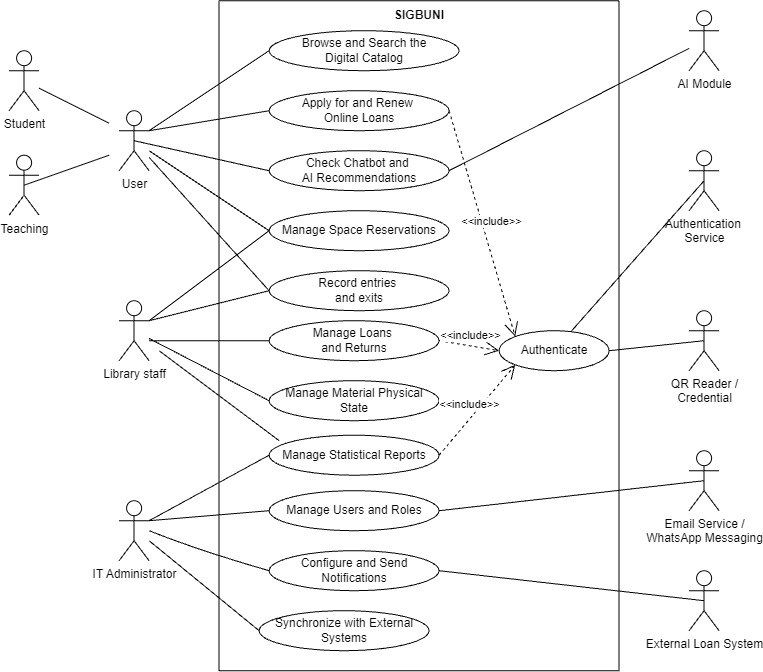
\includegraphics[width=0.82\textwidth]{imagenes/Diagrama_de_Caso_de_Usos.png}
\caption{Diagrama general de casos de uso.}
\end{figure}

\subsection{Especificación textual de casos de uso}
\caseblock{CU-01}{Consultar catálogo digital}{Estudiante / docente / bibliotecario}{Identificar materiales disponibles para estudio o investigación.}{Usuario autenticado o acceso permitido al catálogo.}{El usuario ingresa un criterio de búsqueda; el sistema consulta el catálogo; el sistema presenta resultados; el usuario selecciona un material; el sistema muestra detalles y estado.}{Si no existen coincidencias, el sistema informa la situación y sugiere modificar los filtros.}{El usuario visualiza materiales y disponibilidad actualizada.}{RF-06, RF-07, RF-08}
\caseblock{CU-02}{Registrar préstamo bibliográfico}{Personal administrativo de biblioteca}{Formalizar la salida de un material bibliográfico a nombre de un usuario autorizado.}{Usuario registrado; material disponible; bibliotecario autenticado.}{El bibliotecario ingresa el usuario; el sistema valida su estado; el bibliotecario ingresa el material; el sistema verifica disponibilidad; el sistema registra el préstamo y actualiza el inventario.}{Si el usuario está bloqueado o el material no está disponible, el sistema cancela el registro e informa el motivo.}{Préstamo registrado y material en estado prestado.}{RF-01, RF-04, RF-05}
\caseblock{CU-03}{Reservar espacio bibliotecario}{Estudiante / docente}{Permitir que un usuario reserve un cubículo, sala u otro espacio disponible.}{Usuario autenticado; espacio registrado en el sistema.}{El usuario selecciona fecha y horario; el sistema muestra disponibilidad; el usuario selecciona un espacio; el sistema valida las reglas; el sistema confirma la reserva.}{Si no hay disponibilidad o se incumple una regla, el sistema muestra alternativas.}{Reserva confirmada y visible en la agenda.}{RF-09, RF-10, RF-11}
\caseblock{CU-04}{Registrar acceso a biblioteca}{Personal de seguridad / sistema}{Registrar el ingreso y la salida de usuarios para control de aforo y trazabilidad.}{Usuario con credencial válida; dispositivo de acceso operativo.}{El usuario presenta su credencial; el sistema valida la identidad; el sistema registra la entrada; al salir, el sistema registra la salida y calcula la permanencia.}{Si la credencial no es válida, el sistema rechaza el registro e informa al operador.}{Acceso registrado para reportes de aforo y visita.}{RF-12, RF-13, RF-18}
\caseblock{CU-05}{Consultar chatbot IA}{Estudiante / docente}{Orientar al usuario sobre servicios, disponibilidad, recomendaciones y procesos bibliotecarios.}{Usuario autenticado; módulo de IA disponible.}{El usuario escribe una pregunta; el sistema interpreta la intención; el chatbot responde; si aplica, sugiere materiales o guía al módulo correspondiente.}{Si el sistema no comprende la pregunta, solicita reformularla o muestra opciones de ayuda.}{El usuario recibe orientación o una recomendación inicial.}{RF-14, RF-15, RF-16, RF-20}
\caseblock{CU-06}{Generar reportes estadísticos}{Bibliotecario / directivo académico}{Obtener información consolidada para la gestión y la toma de decisiones.}{Usuario con rol autorizado; existencia de registros históricos.}{El usuario selecciona el tipo de reporte y rango de fechas; el sistema procesa los datos; el sistema muestra indicadores; el usuario descarga o visualiza el reporte.}{Si no hay datos suficientes, el sistema muestra un reporte vacío con advertencia.}{Reporte generado para análisis institucional.}{RF-18}

\blankcase{CU-07}{Gestionar usuarios, roles y permisos}
\blankcase{CU-08}{Enviar comunicados masivos}
\blankcase{CU-09}{Registrar devolución de material}
\blankcase{CU-10}{Consultar y exportar reportes}

\subsection{Diagrama de clases refinado}
El modelo disponible es conceptual y contiene atributos, pero no documenta operaciones completas para todas las clases. Debe conservarse como línea base y reemplazarse por una versión refinada con visibilidades, tipos, operaciones, multiplicidades y restricciones.
\begin{figure}[H]\centering
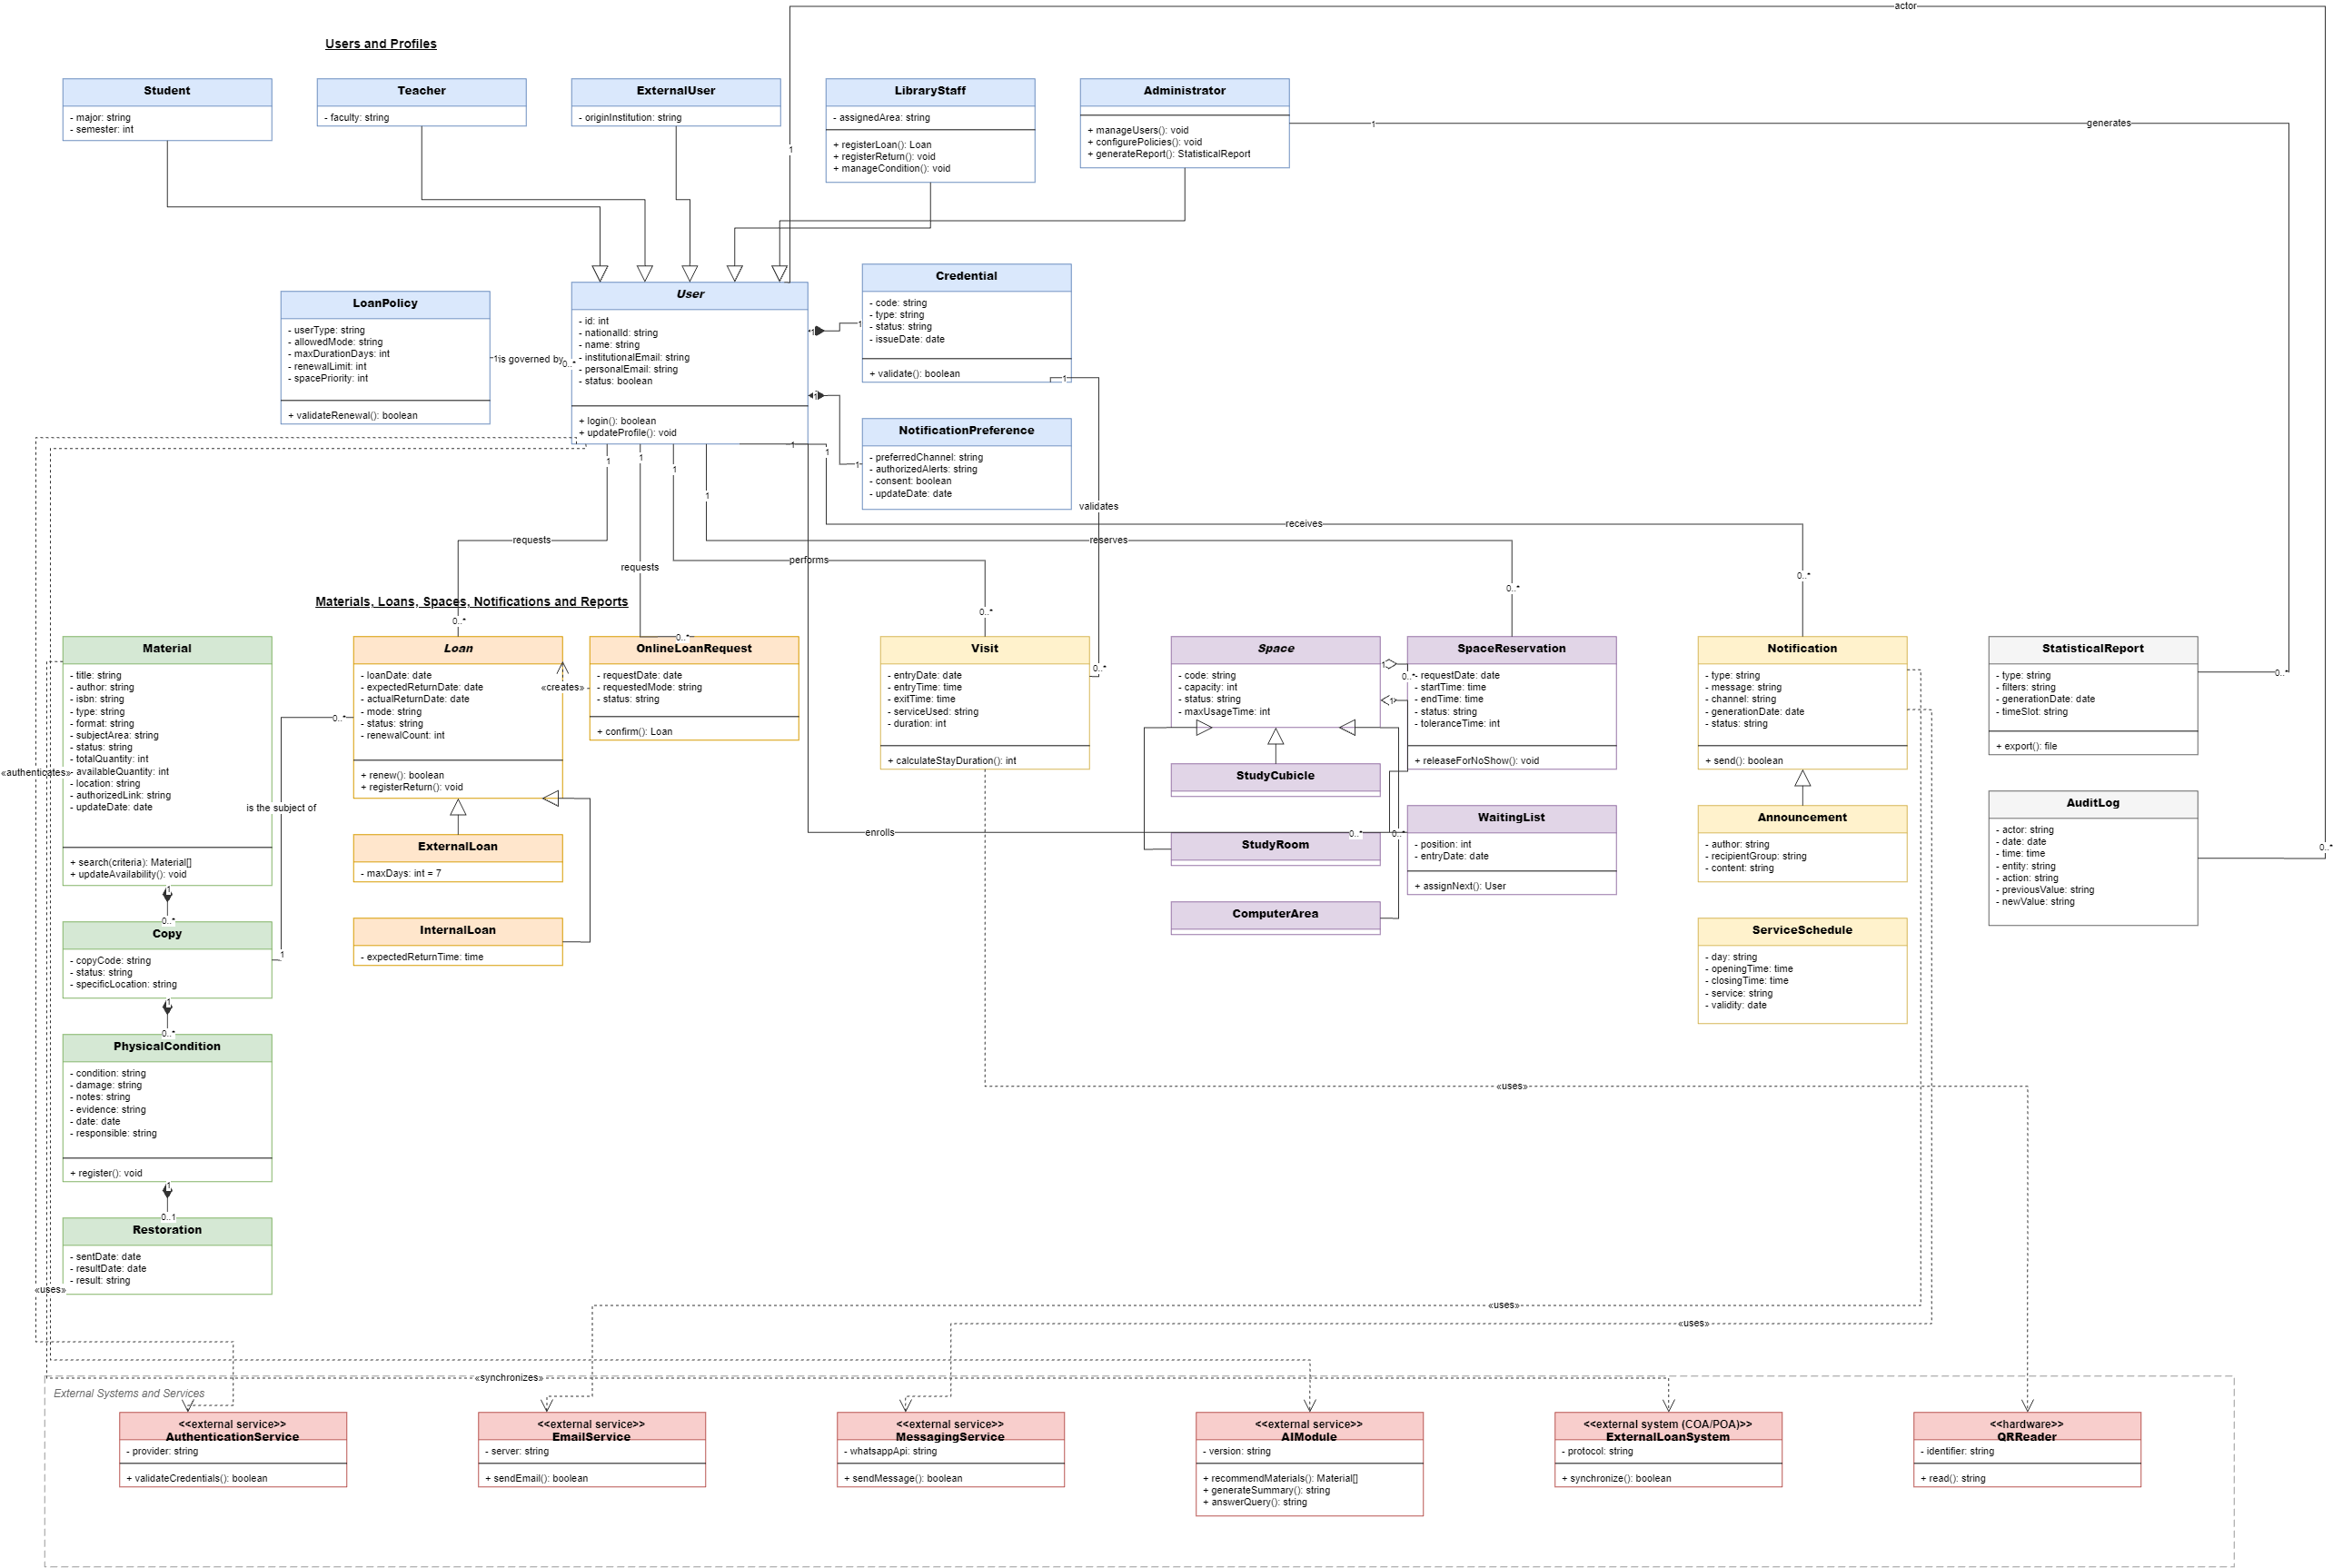
\includegraphics[height=0.78\textheight]{diagrama_clases_conceptual.png}
\caption{Diagrama de clases conceptual heredado de la Entrega 2 (1B).}
\end{figure}
\placeholderfigure{Diagrama de clases refinado con atributos y operaciones}{8cm}

\subsection{Diagramas de secuencia para RF Must}
\begin{longtable}{P{0.12\textwidth}P{0.20\textwidth}P{0.48\textwidth}P{0.13\textwidth}}\toprule
\textbf{ID} & \textbf{RF/CU} & \textbf{Archivo esperado} & \textbf{Estado}\\\midrule\endfirsthead
\toprule\textbf{ID} & \textbf{RF/CU} & \textbf{Archivo esperado} & \textbf{Estado}\\\midrule\endhead
DS-01 & RF-01 / \completar & \path{03_Modelado/Diagramas_UML/DS-01_*.png} + fuente editable & \completar\\
DS-02 & RF-02 / \completar & \path{03_Modelado/Diagramas_UML/DS-02_*.png} + fuente editable & \completar\\
DS-03 & RF-04 / \completar & \path{03_Modelado/Diagramas_UML/DS-03_*.png} + fuente editable & \completar\\
DS-04 & RF-05 / \completar & \path{03_Modelado/Diagramas_UML/DS-04_*.png} + fuente editable & \completar\\
DS-05 & RF-06 / \completar & \path{03_Modelado/Diagramas_UML/DS-05_*.png} + fuente editable & \completar\\
DS-06 & RF-07 / \completar & \path{03_Modelado/Diagramas_UML/DS-06_*.png} + fuente editable & \completar\\
DS-07 & RF-08 / \completar & \path{03_Modelado/Diagramas_UML/DS-07_*.png} + fuente editable & \completar\\
DS-08 & RF-09 / \completar & \path{03_Modelado/Diagramas_UML/DS-08_*.png} + fuente editable & \completar\\
DS-09 & RF-10 / \completar & \path{03_Modelado/Diagramas_UML/DS-09_*.png} + fuente editable & \completar\\
DS-10 & RF-12 / \completar & \path{03_Modelado/Diagramas_UML/DS-10_*.png} + fuente editable & \completar\\
DS-11 & RF-13 / \completar & \path{03_Modelado/Diagramas_UML/DS-11_*.png} + fuente editable & \completar\\
DS-12 & RF-17 / \completar & \path{03_Modelado/Diagramas_UML/DS-12_*.png} + fuente editable & \completar\\
DS-13 & RF-18 / \completar & \path{03_Modelado/Diagramas_UML/DS-13_*.png} + fuente editable & \completar\\
\bottomrule\end{longtable}
\placeholderfigure{Plantilla para diagrama de secuencia}{7cm}

\subsection{Diagramas de actividad para flujos principales}
\begin{longtable}{P{0.12\textwidth}P{0.20\textwidth}P{0.48\textwidth}P{0.13\textwidth}}\toprule
\textbf{ID} & \textbf{RF/CU} & \textbf{Archivo esperado} & \textbf{Estado}\\\midrule\endfirsthead
\toprule\textbf{ID} & \textbf{RF/CU} & \textbf{Archivo esperado} & \textbf{Estado}\\\midrule\endhead
DA-01 & RF-01 / \completar & \path{03_Modelado/Diagramas_UML/DA-01_*.png} + fuente editable & \completar\\
DA-02 & RF-02 / \completar & \path{03_Modelado/Diagramas_UML/DA-02_*.png} + fuente editable & \completar\\
DA-03 & RF-04 / \completar & \path{03_Modelado/Diagramas_UML/DA-03_*.png} + fuente editable & \completar\\
DA-04 & RF-05 / \completar & \path{03_Modelado/Diagramas_UML/DA-04_*.png} + fuente editable & \completar\\
DA-05 & RF-06 / \completar & \path{03_Modelado/Diagramas_UML/DA-05_*.png} + fuente editable & \completar\\
DA-06 & RF-07 / \completar & \path{03_Modelado/Diagramas_UML/DA-06_*.png} + fuente editable & \completar\\
DA-07 & RF-08 / \completar & \path{03_Modelado/Diagramas_UML/DA-07_*.png} + fuente editable & \completar\\
DA-08 & RF-09 / \completar & \path{03_Modelado/Diagramas_UML/DA-08_*.png} + fuente editable & \completar\\
DA-09 & RF-10 / \completar & \path{03_Modelado/Diagramas_UML/DA-09_*.png} + fuente editable & \completar\\
DA-10 & RF-12 / \completar & \path{03_Modelado/Diagramas_UML/DA-10_*.png} + fuente editable & \completar\\
DA-11 & RF-13 / \completar & \path{03_Modelado/Diagramas_UML/DA-11_*.png} + fuente editable & \completar\\
DA-12 & RF-17 / \completar & \path{03_Modelado/Diagramas_UML/DA-12_*.png} + fuente editable & \completar\\
DA-13 & RF-18 / \completar & \path{03_Modelado/Diagramas_UML/DA-13_*.png} + fuente editable & \completar\\
\bottomrule\end{longtable}
\placeholderfigure{Plantilla para diagrama de actividad}{7cm}

\subsection{Diagramas de estados}
\placeholderfigure{Diagrama de estados de MaterialBibliográfico}{6cm}
\placeholderfigure{Diagrama de estados de Préstamo}{6cm}
\placeholderfigure{Diagrama de estados de ReservaEspacio}{6cm}

\subsection{Diagrama de componentes}
\placeholderfigure{Diagrama de componentes de SIGBUNI}{7cm}

\subsection{Diagrama de despliegue}
\placeholderfigure{Diagrama de despliegue de SIGBUNI}{7cm}

\section{Priorización y trazabilidad extendida}
\subsection{Priorización MoSCoW, Kano y WSJF}
La clasificación MoSCoW proviene de la Entrega 2 (1B). Kano y WSJF requieren nueva valoración con stakeholders; sus celdas permanecen pendientes.

\begin{longtable}{P{0.10\textwidth}P{0.16\textwidth}P{0.16\textwidth}P{0.18\textwidth}P{0.32\textwidth}}\toprule
\textbf{RF} & \textbf{MoSCoW} & \textbf{Kano} & \textbf{WSJF} & \textbf{Justificación/evidencia}\\\midrule\endfirsthead
\toprule\textbf{RF} & \textbf{MoSCoW} & \textbf{Kano} & \textbf{WSJF} & \textbf{Justificación/evidencia}\\\midrule\endhead
RF-01 & Must & \completar & \completar & EV-01, EV-15\\
RF-02 & Must & \completar & \completar & EV-01\\
RF-03 & Should & \completar & \completar & EV-10\\
RF-04 & Must & \completar & \completar & EV-01, EV-08\\
RF-05 & Must & \completar & \completar & EV-01\\
RF-06 & Must & \completar & \completar & EV-02, EV-13\\
RF-07 & Must & \completar & \completar & EV-02\\
RF-08 & Must & \completar & \completar & EV-02\\
RF-09 & Must & \completar & \completar & EV-03, EV-15\\
RF-10 & Must & \completar & \completar & EV-03\\
RF-11 & Should & \completar & \completar & EV-03\\
RF-12 & Must & \completar & \completar & EV-04\\
RF-13 & Must & \completar & \completar & EV-04\\
RF-14 & Should & \completar & \completar & EV-05\\
RF-15 & Should & \completar & \completar & EV-05\\
RF-16 & Could & \completar & \completar & EV-06\\
RF-17 & Must & \completar & \completar & EV-09\\
RF-18 & Must & \completar & \completar & EV-07, EV-14\\
RF-19 & Should & \completar & \completar & EV-11\\
RF-20 & Could & \completar & \completar & EV-12\\
RF-21 & \completar & \completar & \completar & \completar\\
RF-22 & \completar & \completar & \completar & \completar\\
RF-23 & \completar & \completar & \completar & \completar\\
RF-24 & \completar & \completar & \completar & \completar\\
RF-25 & \completar & \completar & \completar & \completar\\
\bottomrule\end{longtable}

\subsection{Matriz de trazabilidad extendida}
La matriz debe contener como mínimo 40 filas y enlazar Ley $\rightarrow$ Objetivo $\rightarrow$ Stakeholder $\rightarrow$ EV $\rightarrow$ RF/RNF/RD $\rightarrow$ CU $\rightarrow$ HU $\rightarrow$ CA $\rightarrow$ Componente $\rightarrow$ Mockup. Las primeras 20 filas reutilizan la trazabilidad previa; las restantes son plantillas.

\begin{landscape}
\tiny
\begin{longtable}{P{0.9cm}P{1.0cm}P{0.8cm}P{1.0cm}P{1.1cm}P{1.0cm}P{1.0cm}P{0.7cm}P{0.9cm}P{0.9cm}P{0.9cm}P{1.2cm}P{1.1cm}}
\toprule
\textbf{ID} & \textbf{Ley/Art.} & \textbf{Obj.} & \textbf{Stake.} & \textbf{EV} & \textbf{Req.} & \textbf{Tipo} & \textbf{CU} & \textbf{HU} & \textbf{CA} & \textbf{Comp.} & \textbf{Mockup} & \textbf{Estado}\\\midrule\endfirsthead
\toprule
\textbf{ID} & \textbf{Ley/Art.} & \textbf{Obj.} & \textbf{Stake.} & \textbf{EV} & \textbf{Req.} & \textbf{Tipo} & \textbf{CU} & \textbf{HU} & \textbf{CA} & \textbf{Comp.} & \textbf{Mockup} & \textbf{Estado}\\\midrule\endhead
MT-001 &  & OBJ-01 & S-03 & EV-01 & RF-01 & RF & CU-02 &  &  & CMP-PRE & MU-05 & Parcial\\
MT-002 &  & OBJ-01 & S-03 & EV-01 & RF-02 & RF & CU-02 &  &  & CMP-PRE & MU-05 & Parcial\\
MT-003 &  & OBJ-01 & S-01 & EV-10 & RF-03 & RF & CU-02 &  &  & CMP-PRE &  & Parcial\\
MT-004 &  & OBJ-01 & S-01 & EV-01/08 & RF-04 & RF & CU-02 &  &  & CMP-NOT & MU-04 & Parcial\\
MT-005 &  & OBJ-01 & S-03 & EV-01 & RF-05 & RF & CU-02 &  &  & CMP-NOT & MU-05 & Parcial\\
MT-006 &  & OBJ-04 & S-01 & EV-02/13 & RF-06 & RF & CU-01 &  &  & CMP-CAT & MU-02 & Parcial\\
MT-007 &  & OBJ-04 & S-01 & EV-02 & RF-07 & RF & CU-01 &  &  & CMP-CAT & MU-02 & Parcial\\
MT-008 &  & OBJ-04 & S-01 & EV-02 & RF-08 & RF & CU-01 &  &  & CMP-CAT & MU-02 & Parcial\\
MT-009 &  & OBJ-02 & S-01 & EV-03/15 & RF-09 & RF & CU-03 &  &  & CMP-RES & MU-03 & Parcial\\
MT-010 &  & OBJ-02 & S-01 & EV-03 & RF-10 & RF & CU-03 &  &  & CMP-RES & MU-03 & Parcial\\
MT-011 &  & OBJ-02 & S-03 & EV-03 & RF-11 & RF & CU-03 &  &  & CMP-RES & MU-03 & Parcial\\
MT-012 &  & OBJ-03 & S-03 & EV-04 & RF-12 & RF & CU-04 &  &  & CMP-ACC &  & Parcial\\
MT-013 &  & OBJ-03 & S-03 & EV-04 & RF-13 & RF & CU-04 &  &  & CMP-ACC &  & Parcial\\
MT-014 &  & OBJ-05 & S-01 & EV-05 & RF-14 & RF & CU-05 &  &  & CMP-IA & MU-04 & Parcial\\
MT-015 &  & OBJ-05 & S-01 & EV-05 & RF-15 & RF & CU-05 &  &  & CMP-IA & MU-04 & Parcial\\
MT-016 &  & OBJ-05 & S-01 & EV-06 & RF-16 & RF & CU-05 &  &  & CMP-IA & MU-04 & Parcial\\
MT-017 &  & OBJ-06 & S-05 & EV-09 & RF-17 & RF & CU-07 &  &  & CMP-ADM & MU-05 & Parcial\\
MT-018 &  & OBJ-06 & S-04 & EV-07/14 & RF-18 & RF & CU-06 &  &  & CMP-REP & MU-05 & Parcial\\
MT-019 &  & OBJ-06 & S-03 & EV-11 & RF-19 & RF & CU-08 &  &  & CMP-NOT & MU-05 & Parcial\\
MT-020 &  & OBJ-05 & S-01 & EV-12 & RF-20 & RF & CU-05 &  &  & CMP-IA & MU-04 & Parcial\\
MT-021 & -- & -- & -- & -- & -- & -- & -- & -- & -- & -- & -- & Pendiente\\
MT-022 & -- & -- & -- & -- & -- & -- & -- & -- & -- & -- & -- & Pendiente\\
MT-023 & -- & -- & -- & -- & -- & -- & -- & -- & -- & -- & -- & Pendiente\\
MT-024 & -- & -- & -- & -- & -- & -- & -- & -- & -- & -- & -- & Pendiente\\
MT-025 & -- & -- & -- & -- & -- & -- & -- & -- & -- & -- & -- & Pendiente\\
MT-026 & -- & -- & -- & -- & -- & -- & -- & -- & -- & -- & -- & Pendiente\\
MT-027 & -- & -- & -- & -- & -- & -- & -- & -- & -- & -- & -- & Pendiente\\
MT-028 & -- & -- & -- & -- & -- & -- & -- & -- & -- & -- & -- & Pendiente\\
MT-029 & -- & -- & -- & -- & -- & -- & -- & -- & -- & -- & -- & Pendiente\\
MT-030 & -- & -- & -- & -- & -- & -- & -- & -- & -- & -- & -- & Pendiente\\
MT-031 & -- & -- & -- & -- & -- & -- & -- & -- & -- & -- & -- & Pendiente\\
MT-032 & -- & -- & -- & -- & -- & -- & -- & -- & -- & -- & -- & Pendiente\\
MT-033 & -- & -- & -- & -- & -- & -- & -- & -- & -- & -- & -- & Pendiente\\
MT-034 & -- & -- & -- & -- & -- & -- & -- & -- & -- & -- & -- & Pendiente\\
MT-035 & -- & -- & -- & -- & -- & -- & -- & -- & -- & -- & -- & Pendiente\\
MT-036 & -- & -- & -- & -- & -- & -- & -- & -- & -- & -- & -- & Pendiente\\
MT-037 & -- & -- & -- & -- & -- & -- & -- & -- & -- & -- & -- & Pendiente\\
MT-038 & -- & -- & -- & -- & -- & -- & -- & -- & -- & -- & -- & Pendiente\\
MT-039 & -- & -- & -- & -- & -- & -- & -- & -- & -- & -- & -- & Pendiente\\
MT-040 & -- & -- & -- & -- & -- & -- & -- & -- & -- & -- & -- & Pendiente\\
\bottomrule
\end{longtable}
\normalsize
\end{landscape}

\section{Producto Mínimo Viable funcional}
\subsection{Repositorio y alcance}
\textbf{Repositorio Git separado del MVP:} \pendiente{agregar URL pública y commit evaluado}.\\
\textbf{Tecnologías y arquitectura:} \pendiente{documentar lenguaje, framework, base de datos, servicios y versión}.\\
\textbf{README de despliegue:} \pendiente{agregar instrucciones reproducibles, por ejemplo Docker Compose o equivalente}.

\subsection{Cobertura de RF Must}
\begin{longtable}{P{0.10\textwidth}P{0.36\textwidth}P{0.15\textwidth}P{0.31\textwidth}}\toprule
\textbf{RF} & \textbf{Funcionalidad} & \textbf{Implementado} & \textbf{Evidencia de ejecución/commit}\\\midrule\endfirsthead
\toprule\textbf{RF} & \textbf{Funcionalidad} & \textbf{Implementado} & \textbf{Evidencia de ejecución/commit}\\\midrule\endhead
RF-01 & Registrar préstamo bibliográfico & \completar & \completar\\
RF-02 & Registrar devolución de material & \completar & \completar\\
RF-04 & Enviar notificación de vencimiento & \completar & \completar\\
RF-05 & Generar alerta por material vencido & \completar & \completar\\
RF-06 & Consultar catálogo digital & \completar & \completar\\
RF-07 & Buscar material por filtros & \completar & \completar\\
RF-08 & Mostrar estado del material & \completar & \completar\\
RF-09 & Reservar espacio bibliotecario & \completar & \completar\\
RF-10 & Mostrar disponibilidad de espacios & \completar & \completar\\
RF-12 & Registrar ingreso a biblioteca & \completar & \completar\\
RF-13 & Registrar salida de biblioteca & \completar & \completar\\
RF-17 & Gestionar usuarios, roles y permisos & \completar & \completar\\
RF-18 & Generar reportes estadísticos & \completar & \completar\\
\bottomrule\end{longtable}
\textbf{Cobertura calculada:} \pendiente{número de RF Must implementados / número total de RF Must; debe ser al menos 60\%}.

\subsection{Demostración funcional}
\textbf{Video menor o igual a 3 minutos:} \pendiente{\path{05_MVP/video_demo.mp4}}.\\
\textbf{Capturas verificables:} \pendiente{insertar capturas producidas por la versión identificada del MVP}.

\section{Trabajo de campo extendido y validación}
\subsection{Inventario mínimo de evidencias}
\begin{longtable}{P{0.25\textwidth}P{0.18\textwidth}P{0.30\textwidth}P{0.20\textwidth}}\toprule
\textbf{Evidencia} & \textbf{Mínimo del corte} & \textbf{Ubicación} & \textbf{Estado verificado}\\\midrule\endfirsthead
\toprule\textbf{Evidencia} & \textbf{Mínimo del corte} & \textbf{Ubicación} & \textbf{Estado verificado}\\\midrule\endhead
Consentimientos firmados & $\geq 8$ para C7; avance hacia 16 & \path{02_Evidencias/Consentimientos/} & \completar\\
Videos de entrevistas & $\geq 6$ para C7; avance hacia 16 & \path{02_Evidencias/Video/} & \completar\\
Audios redundantes & $\geq 6$ para C7; avance hacia 16 & \path{02_Evidencias/Audio/} & \completar\\
Fotos del entorno & $\geq 15$ para C7; meta extendida 20 & \path{02_Evidencias/Fotos_Entorno/} & \completar\\
Fotos de aplicación del cuestionario & $\geq 5$ & \path{02_Evidencias/Cuestionario/Fotos_Aplicacion/} & \completar\\
Respuestas del cuestionario & $n\geq 30$ para gatekeeper; meta $n\geq 60$ por perfil & \path{02_Evidencias/Cuestionario/Respuestas/} & \completar\\
Documentos de la organización & $\geq 3$ para C7; meta 5 & \path{02_Evidencias/Documentos_Organizacion/} & \completar\\
Walkthrough de validación & $\geq 3$ para C7; meta 6 & \path{02_Evidencias/Validacion_Walkthrough/} & \completar\\
Codificación temática y saturación & Tabla completa + curva & \path{02_Evidencias/Codificacion_Tematica/} & \completar\\\bottomrule
\end{longtable}

\subsection{Evidencia heredada documentada}
Las Entregas previas muestran trabajo de campo y registran entrevistas, encuesta y fotografías. Estas imágenes se incluyen solo como referencia histórica; no sustituyen los nuevos consentimientos ni la segunda ronda requerida.
\begin{figure}[H]\centering
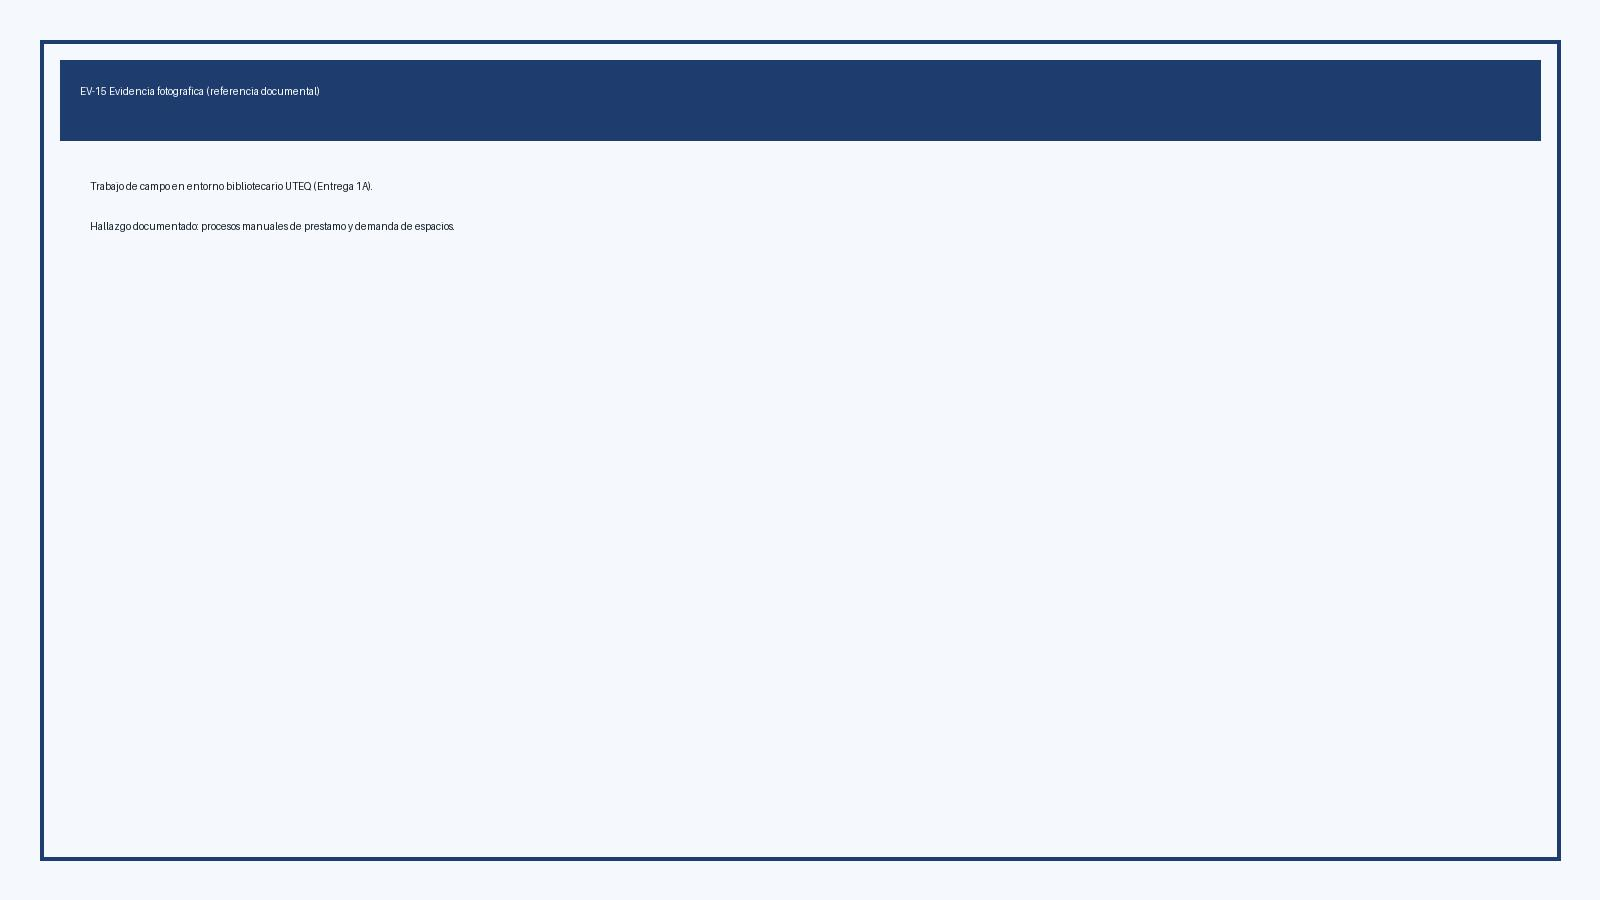
\includegraphics[height=0.42\textheight]{EV-15_trabajo_campo_01.jpg}\hfill
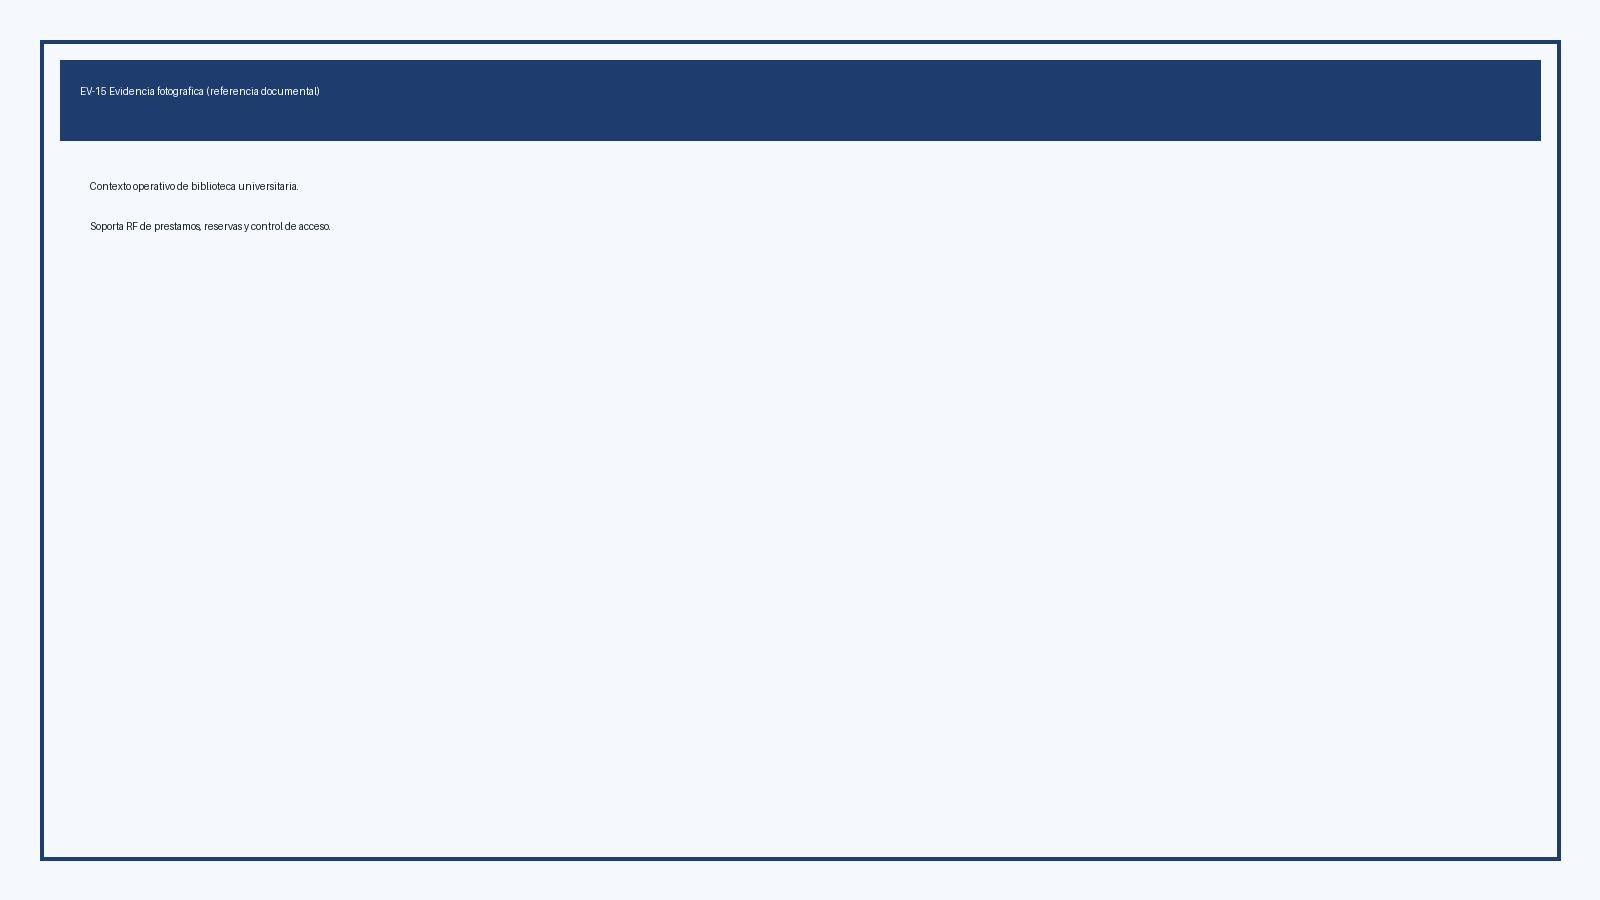
\includegraphics[height=0.42\textheight]{EV-15_trabajo_campo_02.jpg}
\caption{Evidencia fotográfica heredada de la Entrega 1A (EV-15).}
\end{figure}

\subsection{Segunda ronda de elicitación}
\textbf{Participantes y perfiles:} \completar.\\
\textbf{Guion de entrevista v2.0:} \completar.\\
\textbf{Cuestionario v2.0:} \completar.\\
\textbf{Criterios de inclusión y exclusión:} \completar.\\
\textbf{Consentimiento actualizado para publicación anonimizada:} \completar.

\subsection{Validación walkthrough}
\begin{longtable}{P{0.12\textwidth}P{0.20\textwidth}P{0.18\textwidth}P{0.20\textwidth}P{0.22\textwidth}}\toprule
\textbf{Sesión} & \textbf{Perfil} & \textbf{Fecha} & \textbf{Requisitos revisados} & \textbf{Acta/video}\\\midrule\endfirsthead
\toprule\textbf{Sesión} & \textbf{Perfil} & \textbf{Fecha} & \textbf{Requisitos revisados} & \textbf{Acta/video}\\\midrule\endhead
VW-01 & Técnico & \completar & \completar & \completar\\
VW-02 & Técnico & \completar & \completar & \completar\\
VW-03 & Técnico & \completar & \completar & \completar\\
VW-04 & No técnico & \completar & \completar & \completar\\
VW-05 & No técnico & \completar & \completar & \completar\\
VW-06 & No técnico & \completar & \completar & \completar\\\bottomrule
\end{longtable}

\subsection{Codificación temática y curva de saturación}
\begin{table}[H]\centering
\caption{Plantilla de codificación temática}
\begin{tabularx}{\textwidth}{P{0.20\textwidth}P{0.14\textwidth}P{0.16\textwidth}P{0.16\textwidth}P{0.14\textwidth}Y}\toprule
\textbf{Fragmento} & \textbf{Código} & \textbf{Categoría} & \textbf{Requisito} & \textbf{EV} & \textbf{Analista}\\\midrule
\completar & \completar & \completar & \completar & \completar & \completar\\\bottomrule
\end{tabularx}
\end{table}
\placeholderfigure{Curva de saturación: códigos nuevos por entrevista}{7cm}

\section{Componente empírico: protocolo experimental}
\subsection{Selección del enfoque}
La guía permite elegir un solo enfoque: (1) comparar calidad de RF humanos y generados por LLM; (2) detectar ambigüedad y smells; o (3) elicitar y validar requisitos de explicabilidad. SIGBUNI contiene módulos de IA, pero el equipo debe declarar y registrar formalmente su decisión antes de recolectar datos.

\textbf{Enfoque seleccionado:} \pendiente{1, 2 o 3}.\\
\textbf{Justificación basada en evidencia y literatura:} \completar.\\
\textbf{URL y fecha del registro OSF previo:} \completar.

\subsection{Preguntas de investigación mediante PICOC}
\begin{table}[H]\centering
\caption{Marco PICOC}
\begin{tabularx}{\textwidth}{P{0.18\textwidth}Y}\toprule
Población & \completar\\
Intervención & \completar\\
Comparación & \completar\\
Resultado (Outcome) & \completar\\
Contexto & SIGBUNI y servicios de biblioteca universitaria de la UTEQ; precisar alcance empírico.\\\bottomrule
\end{tabularx}
\end{table}

\begin{enumerate}[label=RQ\arabic*:]
\item \completar.
\item \completar.
\item \completar.
\end{enumerate}

\subsection{Hipótesis o proposiciones}
\textbf{H0-1:} \completar.\\
\textbf{H1-1:} \completar.\\
\textbf{H0-2 / H1-2 o proposiciones de estudio de caso:} \completar.

\subsection{Variables}
\begin{longtable}{P{0.20\textwidth}P{0.25\textwidth}P{0.30\textwidth}P{0.18\textwidth}}\toprule
\textbf{Tipo} & \textbf{Variable} & \textbf{Operacionalización} & \textbf{Escala}\\\midrule\endfirsthead
\toprule\textbf{Tipo} & \textbf{Variable} & \textbf{Operacionalización} & \textbf{Escala}\\\midrule\endhead
Independiente & \completar & \completar & \completar\\
Dependiente & \completar & \completar & \completar\\
Control & \completar & \completar & \completar\\\bottomrule
\end{longtable}

\subsection{Participantes, muestreo y ética}
\textbf{Población y muestra:} \completar.\\
\textbf{Cálculo de potencia o justificación de tamaño:} \completar.\\
\textbf{Reclutamiento e inclusión/exclusión:} \completar.\\
\textbf{Consentimiento y anonimización:} \completar.\\
\textbf{Tratamiento de datos conforme a la LOPDP:} \completar.

\subsection{Instrumentos y replicabilidad}
\begin{itemize}
\item Guion de entrevista v2.0: \completar.
\item Cuestionario v2.0: \completar.
\item Rúbrica de evaluación experta: \completar.
\item Prompt exacto del LLM, modelo, versión, temperatura, top-p, top-k y semilla, si aplica: \completar.
\item Plantilla de consentimiento actualizado: \completar.
\end{itemize}

\subsection{Plan de análisis estadístico}
\begin{enumerate}
\item Preparación y validación de datos: \completar.
\item Prueba de normalidad Shapiro--Wilk: \completar.
\item Prueba paramétrica o no paramétrica: \completar.
\item Tamaño del efecto (Cohen $d$ o Cliff $\delta$): \completar.
\item Acuerdo interevaluador (Cohen $\kappa$ / Fleiss $\kappa$), si aplica: \completar.
\item Corrección por comparaciones múltiples: \completar.
\item Scripts reproducibles en R o Python: \completar.
\end{enumerate}

\subsection{Resultados}
\pendiente{No redactar resultados hasta ejecutar el protocolo registrado y generar tablas/figuras desde los scripts versionados.}

\subsection{Amenazas a la validez}
\begin{tabularx}{\textwidth}{P{0.18\textwidth}Y Y}\toprule
\textbf{Categoría} & \textbf{Amenaza} & \textbf{Mitigación y limitación remanente}\\\midrule
Interna & \completar & \completar\\
Externa & \completar & \completar\\
Constructo & \completar & \completar\\
Conclusión & \completar & \completar\\\bottomrule
\end{tabularx}

\section{Preparación de publicación y datos FAIR}
\subsection{Paquete de datos}
El paquete para Zenodo debe incluir transcripciones anonimizadas en JSON, respuestas en CSV, corpus RF/RNF etiquetado, matriz de trazabilidad, prompts y respuestas de LLM cuando apliquen, scripts y un \path{README_dataset.md}. Los principios FAIR se documentarán siguiendo \cite{wilkinson2016fair}.

\begin{longtable}{P{0.30\textwidth}P{0.34\textwidth}P{0.28\textwidth}}\toprule
\textbf{Artefacto} & \textbf{Formato/ubicación} & \textbf{Estado}\\\midrule\endfirsthead
\toprule\textbf{Artefacto} & \textbf{Formato/ubicación} & \textbf{Estado}\\\midrule\endhead
Transcripciones anonimizadas & JSON / \path{07_Publicacion/dataset_zenodo/} & \completar\\
Respuestas de cuestionario & CSV & \completar\\
Corpus RF/RNF & JSON & \completar\\
Matriz de trazabilidad & CSV & \completar\\
Prompts y respuestas LLM & Markdown/JSON, si aplica & \completar\\
Scripts de análisis & R/Python & \completar\\
Diccionario y citación & \path{README_dataset.md} & \completar\\
Licencia & CC BY 4.0 para datos/documento & \completar\\
DOI Zenodo & URL/DOI persistente & \completar\\\bottomrule
\end{longtable}

\subsection{Borrador de manuscrito paralelo}
\textbf{Título preliminar (10--15 palabras):} \completar.\\
\textbf{Resumen preliminar (200--250 palabras; contexto, objetivo, método, resultados y conclusiones):} \pendiente{no incluir resultados hasta disponer de datos}.\\
\textbf{Palabras clave:} \completar.

\subsubsection{Introducción del manuscrito}
\pendiente{cuatro párrafos: caso real, brecha reciente, contribuciones sustentables y RQ/estructura}.

\subsubsection{Trabajo relacionado}
\textbf{Cadena de búsqueda:} \completar.\\
\textbf{Bases consultadas:} Scopus y Google Scholar; agregar fecha y resultados verificables.\\
\textbf{Criterios de inclusión/exclusión:} \completar.\\
\textbf{Cuadro comparativo de 10--15 trabajos:} \completar.

\subsubsection{Metodología}
Debe corresponder exactamente al protocolo registrado en OSF y permitir la replicación.

\subsubsection{Resultados, discusión y conclusiones}
\pendiente{completar exclusivamente después de ejecutar el estudio y analizar los datos con scripts versionados}.

\subsection{Análisis de revistas objetivo}
La selección se realizará con las herramientas oficiales de Springer Nature, Elsevier e IEEE. Los indicadores vigentes deben verificarse en línea al momento del análisis.

\small
\begin{longtable}{P{0.09\textwidth}P{0.18\textwidth}P{0.11\textwidth}P{0.07\textwidth}P{0.09\textwidth}P{0.09\textwidth}P{0.17\textwidth}}\toprule
\textbf{Editorial} & \textbf{Revista} & \textbf{JCR/Q} & \textbf{IF} & \textbf{Modelo} & \textbf{APC} & \textbf{Ajuste/tiempo}\\\midrule\endfirsthead
\toprule\textbf{Editorial} & \textbf{Revista} & \textbf{JCR/Q} & \textbf{IF} & \textbf{Modelo} & \textbf{APC} & \textbf{Ajuste/tiempo}\\\midrule\endhead
Springer & -- & -- & -- & OA & -- & --\\
Springer & -- & -- & -- & Híbrida & -- & --\\
Elsevier & -- & -- & -- & OA & -- & --\\
Elsevier & -- & -- & -- & Híbrida & -- & --\\
IEEE & -- & -- & -- & OA & -- & --\\
IEEE & -- & -- & -- & Híbrida & -- & --\\\bottomrule
\end{longtable}
\normalsize

\subsection{Disponibilidad de datos y materiales}
\textbf{DOI de Zenodo:} \completar.\\
\textbf{Registro OSF:} \completar.\\
\textbf{Licencia del dataset:} CC BY 4.0, una vez aprobada y publicada.\\
\textbf{Citación del software/dataset:} \completar conforme a \cite{smith2016software,druskat2021cff}.

\section{Estructura y verificación del repositorio}
\subsection{Árbol obligatorio}
\begin{Verbatim}[fontsize=\small]
SIGBUNI_ISR401/
  README.md
  LICENSE
  CITATION.cff
  CHANGELOG.md
  .gitignore
  checksums.sha256
  01_ERS/
    ERS_SRS_2A_v1.0.pdf
    ERS_SRS_2A_v1.0.tex
    referencias.bib
  02_Evidencias/
    Consentimientos/ Video/ Audio/ Fotos_Entorno/
    Cuestionario/Fotos_Aplicacion/ Cuestionario/Respuestas/
    Documentos_Organizacion/ Validacion_Walkthrough/
    Codificacion_Tematica/
  03_Modelado/Diagramas_UML/  03_Modelado/Mockups/
  04_Trazabilidad/
    matriz_trazabilidad.csv
    priorizacion_moscow_kano.csv
  05_MVP/README.md  05_MVP/video_demo.mp4
  06_Experimento/
    protocolo.pdf  osf_registration.pdf  instrumentos/
    prompts_llm/ resultados/ scripts_analisis/
  07_Publicacion/
    manuscrito_borrador.pdf  dataset_zenodo/
\end{Verbatim}

\subsection{Archivos raíz obligatorios}
\begin{tabularx}{\textwidth}{P{0.22\textwidth}Y P{0.14\textwidth}}\toprule
\textbf{Archivo} & \textbf{Contenido mínimo} & \textbf{Estado}\\\midrule
README.md & Sistema, integrantes/roles, enlaces, reproducción del experimento y tabla de contenidos. & \completar\\
LICENSE & Licencia del código y CC BY 4.0 para datos/documento. & \completar\\
CITATION.cff & Autores, ORCID, título, versión, fecha y DOI. & \completar\\
CHANGELOG.md & Historial desde 1A. & \completar\\
checksums.sha256 & Hashes de archivos multimedia. & \completar\\\bottomrule
\end{tabularx}

\subsection{Checklist de aceptación y gatekeepers}
\begin{longtable}{P{0.06\textwidth}P{0.78\textwidth}P{0.10\textwidth}}\toprule
\textbf{ID} & \textbf{Comprobación} & \textbf{Estado}\\\midrule\endfirsthead
\toprule\textbf{ID} & \textbf{Comprobación} & \textbf{Estado}\\\midrule\endhead
CK-01 & Estructura de carpetas exacta. & \completar\\
CK-02 & Cinco archivos raíz completos. & \completar\\
CK-03 & PDF unificado, numerado, con historial y enlace GitHub. & \completar\\
CK-04 & Nomenclatura estándar de multimedia. & \completar\\
CK-05 & Audio/video válido con ffprobe y duración mayor a cero. & \completar\\
CK-06 & Consentimientos legibles y firmados. & \completar\\
CK-07 & Cuestionario con fotos y $n\geq30$. & \completar\\
CK-08 & Protocolo OSF registrado antes de ejecutar. & \completar\\
CK-09 & Prompts con parámetros reproducibles, si aplica. & \completar\\
CK-10 & Scripts reproducen tablas y figuras. & \completar\\
CK-11 & Hashes SHA-256 coinciden. & \completar\\
CK-12 & Matriz con al menos 40 filas y columnas obligatorias. & \completar\\
CK-13 & Toda evidencia declarada existe y es verificable. & \completar\\
CK-14 & 25 RF, 15 RNF, 10 CU detallados y explicabilidad IA. & \completar\\
CK-15 & MVP ejecutable con cobertura mínima del 60\% de RF Must. & \completar\\\bottomrule
\end{longtable}

\section{Conclusiones y trabajo pendiente}
La línea base disponible define el contexto de SIGBUNI, seis objetivos, veinte RF, ocho RNF, ocho restricciones, seis CU detallados, cinco mockups, un diagrama de contexto, un diagrama general de casos de uso, un modelo conceptual de clases y una trazabilidad parcial. El documento los conserva y los reorganiza dentro de la estructura solicitada para la Entrega 3 (2A).

Para cumplir la rúbrica aún deben completarse y validarse, como mínimo: cinco RF adicionales, siete RNF con cobertura de las nueve características y explicabilidad, el mapeo legal por artículo, historias Connextra y Gherkin para todos los RF Must, cuatro CU detallados adicionales, los diagramas UML restantes, mockups de alta fidelidad, Kano/WSJF, cuarenta filas completas de trazabilidad, segunda ronda de evidencias, MVP ejecutable, protocolo registrado en OSF y paquete FAIR. Los resultados y la discusión permanecerán vacíos hasta que existan datos primarios y scripts reproducibles.

\appendices
\section{Catálogo inicial de evidencias}
\begin{longtable}{P{0.12\textwidth}P{0.23\textwidth}P{0.45\textwidth}P{0.13\textwidth}}\toprule
\textbf{EV} & \textbf{Técnica/fuente} & \textbf{Hallazgo documentado} & \textbf{Estado}\\\midrule\endfirsthead
\toprule\textbf{EV} & \textbf{Técnica/fuente} & \textbf{Hallazgo documentado} & \textbf{Estado}\\\midrule\endhead
EV-01 & Entrevista & Préstamo manual, devoluciones y vencimientos con seguimiento reactivo. & Verificar archivo.\\
EV-02 & Encuesta & Necesidad de catálogo actualizado, filtros y estado del material. & Verificar archivo.\\
EV-03 & Observación & Reserva informal, alta demanda e inasistencia. & Verificar archivo.\\
EV-04 & Entrevista & Control manual de ingreso y falta de salida digital. & Verificar archivo.\\
EV-05 & Encuesta & Ayuda digital y orientación personalizada. & Verificar archivo.\\
EV-06 & Análisis de problemática & Dificultad para valorar documentos extensos. & Verificar respaldo.\\
EV-07 & Entrevista & Necesidad de reportes de uso. & Verificar archivo.\\
EV-08 & Encuesta & Preferencia por alertas internas. & Verificar archivo.\\
EV-09 & Observación & Necesidad de gestión de usuarios y roles. & Verificar archivo.\\
EV-10 & Encuesta & Preferencia por préstamo digital o mixto. & Verificar archivo.\\
EV-11 & Entrevista & Necesidad de comunicados masivos. & Verificar archivo.\\
EV-12 & Análisis de problemática & Recomendaciones por historial y carrera. & Verificar respaldo.\\
EV-13 & Acta de encuesta & Importancia del acceso desde casa. & Verificar archivo.\\
EV-14 & Acta de entrevista & Control de aforo en horarios críticos. & Verificar archivo.\\
EV-15 & Evidencia fotográfica & Trabajo de campo en entorno bibliotecario. & Incluida como imagen histórica.\\\bottomrule
\end{longtable}

\section{Notas para edición manual}
Todos los marcadores rojos se localizan buscando \texttt{PENDIENTE} o \texttt{COMPLETAR} en el archivo fuente. Las imágenes se cargan desde \texttt{images/}. Para reemplazar una figura sin modificar el código, conserve el mismo nombre del archivo. Para agregar bibliografía, edite \texttt{referencias.bib} y cite con \texttt{\\cite\{clave\}}. Compile con \texttt{latexmk -pdf ERS\_SRS\_2A\_v1.0.tex}.

\nocite{*}
\bibliographystyle{IEEEtran}
\bibliography{referencias}
\end{document}
